\documentclass[]{beamer}
% Class options include: notes, notesonly, handout, trans,
%                        hidesubsections, shadesubsections,
%                        inrow, blue, red, grey, brown

% Theme for beamer presentation.
\usepackage{beamerthemesplit} 
\usepackage{multimedia}
\usepackage{hyperref}

\usepackage{collectbox}

\usepackage[utf8]{inputenc}
\usepackage[english]{babel}

%%%%%%%%%%%%%%%%%%%%%%%%%%%%%%%%%%%%%%%%%%%%%%%%%%%%%%%%%%%%%%%%%%%%%%



\definecolor{mypink1}{rgb}{0.858, 0.188, 0.478}

\newcommand{\mybox}{%
    \collectbox{%
        \setlength{\fboxsep}{1pt}%
        \fbox{\BOXCONTENT}%
    }%
}

%%%%%%%%%%%%%%%%%%%%%%%%%%%%%%%%%%%%%%%%%%%%%%%%%%%%%%%%%%%%%%%%%%%%%%
% Other themes include: beamerthemebars, beamerthemelined, 
%                       beamerthemetree, beamerthemetreebars  

\title{PHY250: STATIC FLUIDS}    % Enter your title between curly braces
\author{Anabela R. Turlione}                 % Enter your name between curly braces
\institute{Digipen}      % Enter your institute name between curly braces
\date{Fall 2022}                    % Enter the date or \today between curly braces


\begin{document}

% Creates title page of slide show using above information
\begin{frame}
  \titlepage
\end{frame}
%\note{Talk for 30 minutes} % Add notes to yourself that will be displayed when
                           % typeset with the notes or notesonly class options

\section[]{}

% Creates table of contents slide incorporating
% all \section and \subsection commands
\begin{frame}
  \tableofcontents
\end{frame}


% \begin{frame}
%   % \centering
%    \movie[externalviewer]{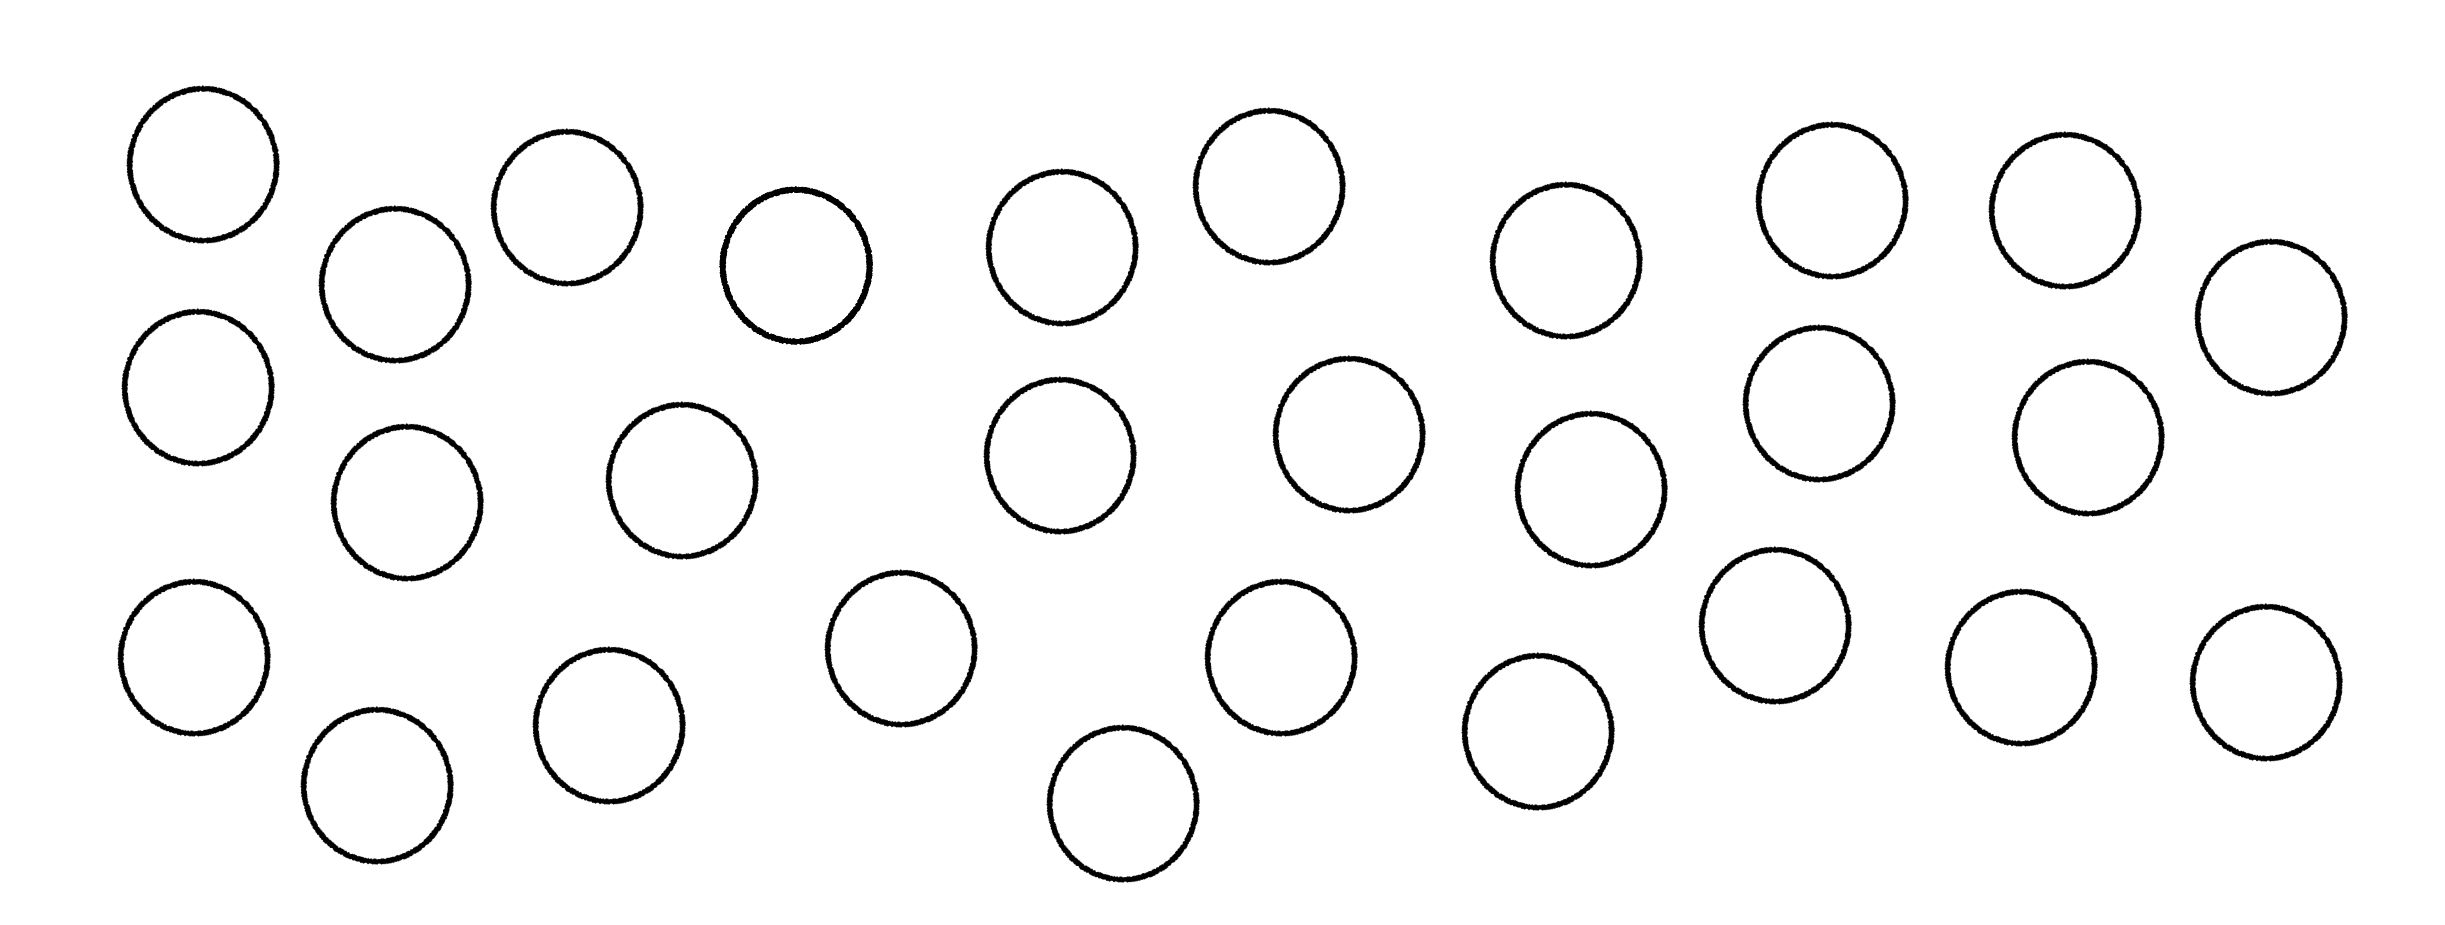
\includegraphics[width=\textheight ,
%    keepaspectratio]{surfacet1.jpg}}{test.mp4}

% \end{frame}
%%%%%%%%%%%%%%%%%%%%%%%%%%%%%%%%%%%%%%%%%%%%%%%%%%%%%%%%%%%%%%%%%%%
\section{Static Fluids}
\subsection{Introduction}

We are going to consider a fluid as a system of particles.

\pause

\begin{frame}
  \frametitle{Fluids}
    \begin{itemize}
      \item  Solid Objects $\rightarrow$ maintain shape except for small amount 
      of elastic deformation.
      \item Fluids $\rightarrow$  materials that are very deformable and can flow.
    \end{itemize}

\pause
\vspace*{10mm}

  We are going to examine \textcolor{mypink1}{Static Fluids} and 
  \textcolor{mypink1}{Dynamic Fluids}.



  \begin{figure}[h!]
    \begin{center}
      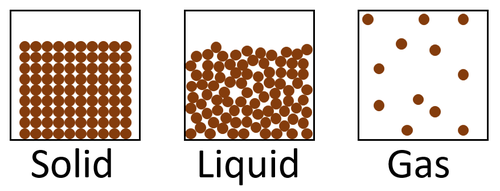
\includegraphics[height=1.3in]{images2/0b.png}
      \label{0b}
    \end{center}
  \end{figure}
  

  
  \end{frame}

%%%%%%%%%%%%%%%%%%%%%%%%%%%%%%%%%%%%%%%%%%%%%%%%%%%%%%%%%%%%%%%



\begin{frame}

\frametitle{Fluids}
\textcolor{mypink1}{Ideal Gases}

\vspace{5mm}

\begin{figure}[h!]
  \begin{center}
    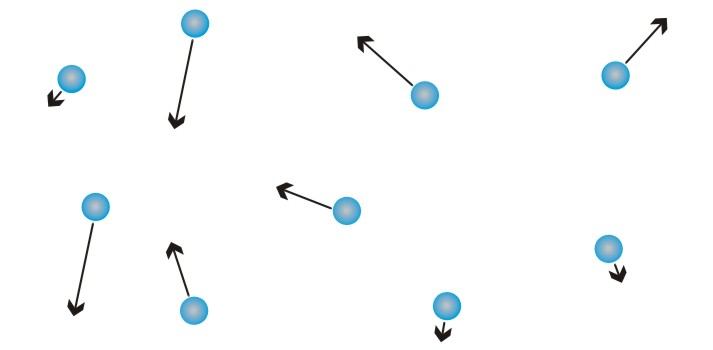
\includegraphics[height=1.1in]{images2/0.jpg}
    \label{0}
  \end{center}
\end{figure}

\begin{itemize}
\item Formed by N point particles that move in straight lines.
\pause
\item They expand to occupy the whole volume of the container.
\pause
\item  They are compressible. 
\pause
\item There is no interaction between the particles.
\pause
\item Elastic collisions, the kinetic energy is conserved. 
\end{itemize}



  
  \end{frame}

%%%%%%%%%%%%%%%%%%%%%%%%%%%%%%%%%%%%%%%%%%%%%%%%%%%%%%%%%%%%%%%

\begin{frame}

    \frametitle{Fluids}
    \textcolor{mypink1}{Liquids: Our Approach}
    
    \begin{figure}[h!]
      \begin{center}
        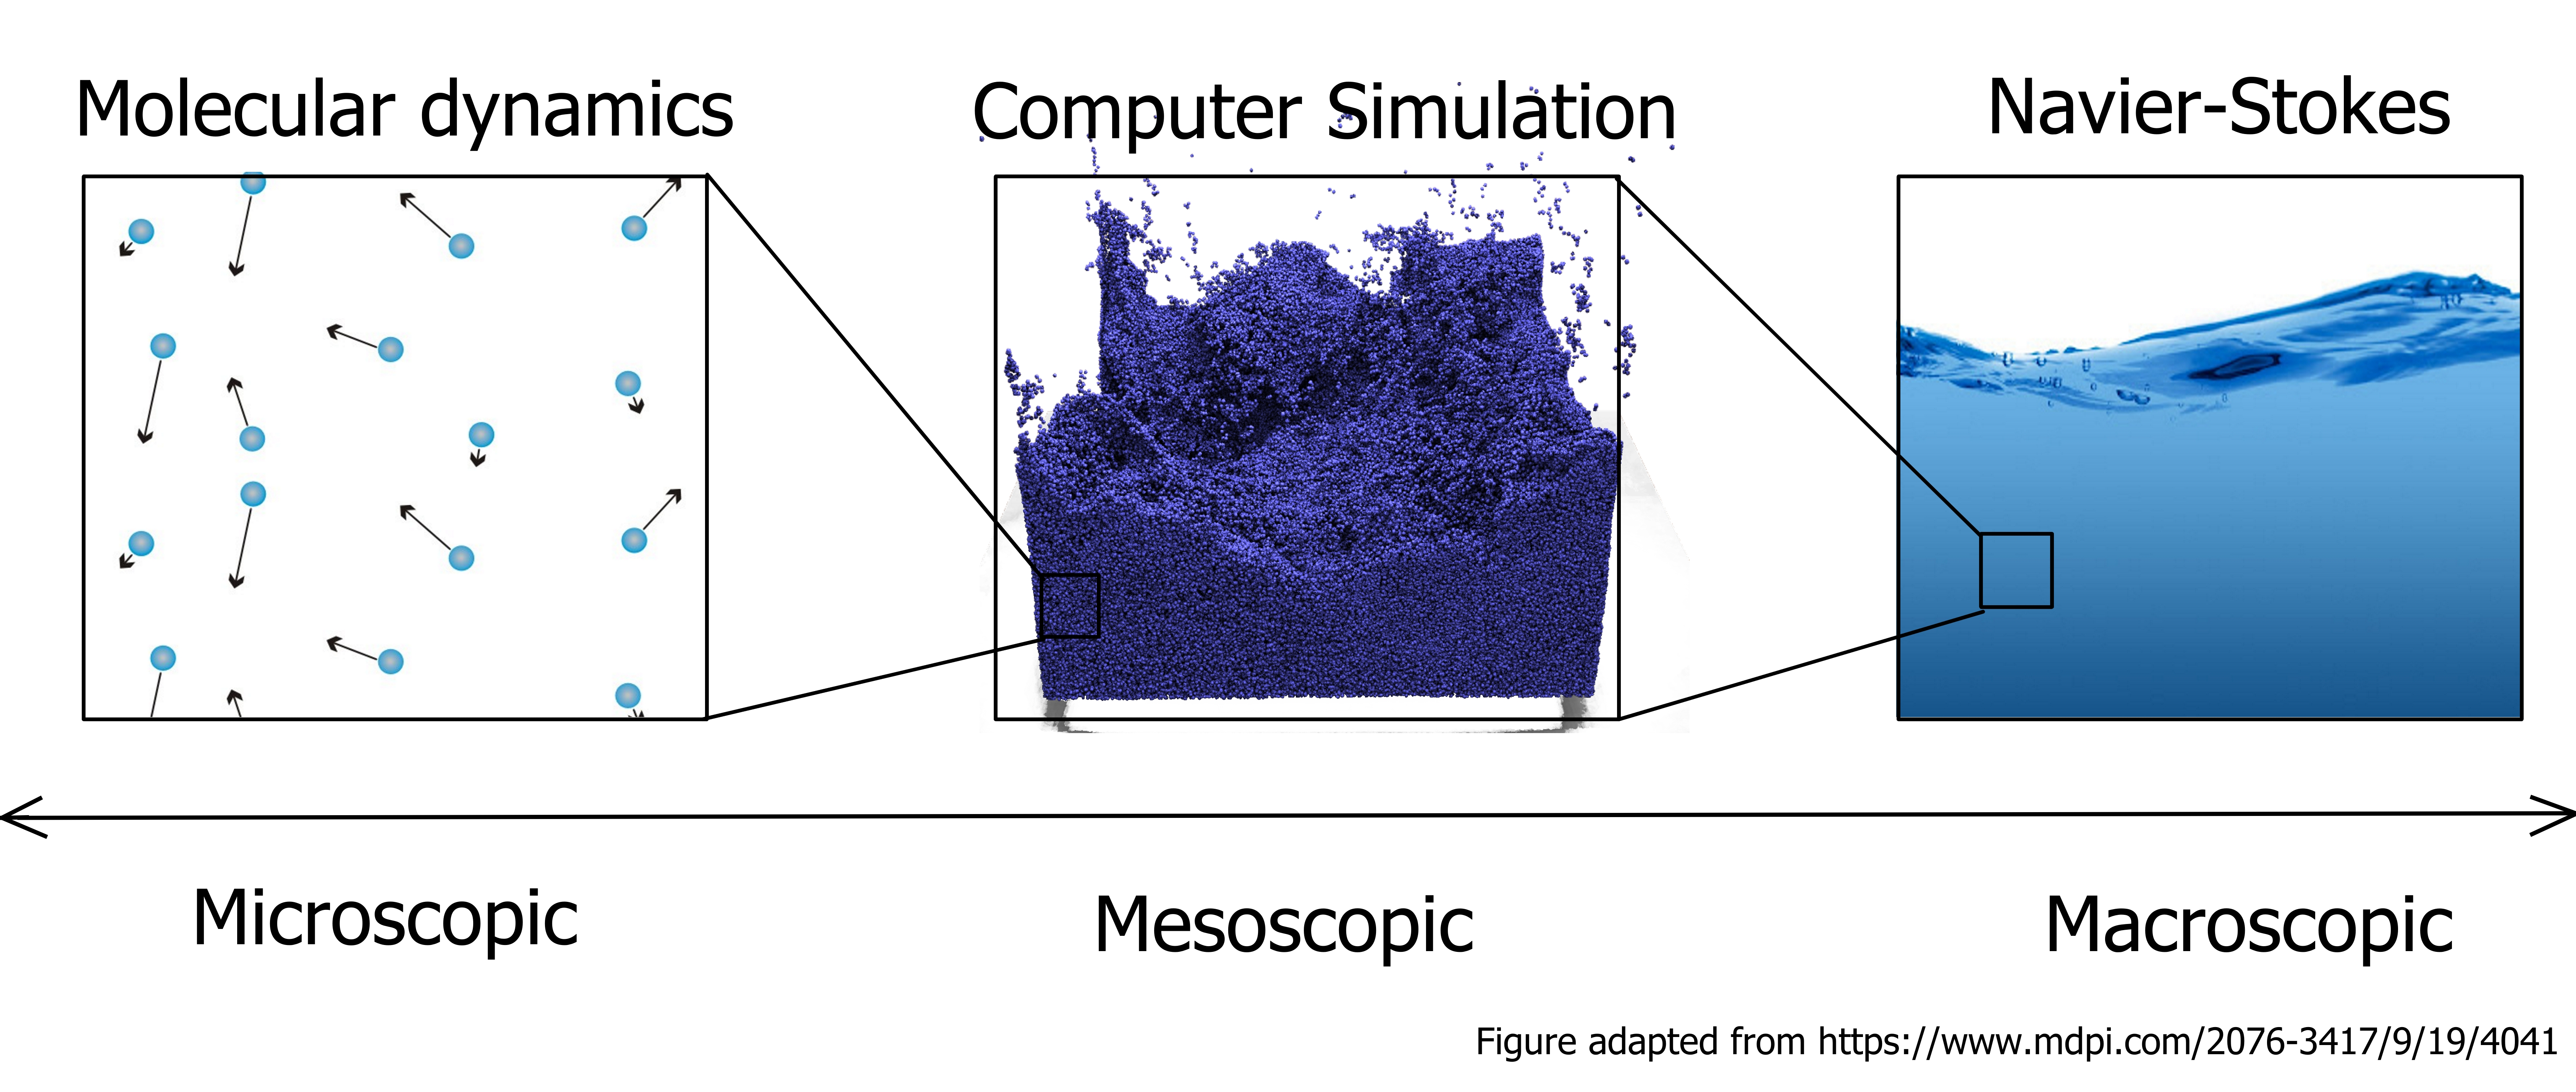
\includegraphics[height=1.8in]{images2/fluids_dimensions.jpg}
        \label{fd}
      \end{center}
    \end{figure}
    
\end{frame}
    
%%%%%%%%%%%%%%%%%%%%%%%%%%%%%%%%%%%%%%%%%%%%%%%%%%%%%%%%%%%%%%%





\begin{frame}

  \frametitle{Fluids}
  \textcolor{mypink1}{Liquids}
  
  \begin{columns}[c]
    \column{2in}  % slides are 3in high by 5in wide
  
  
    \begin{figure}[h!]
      \begin{center}
        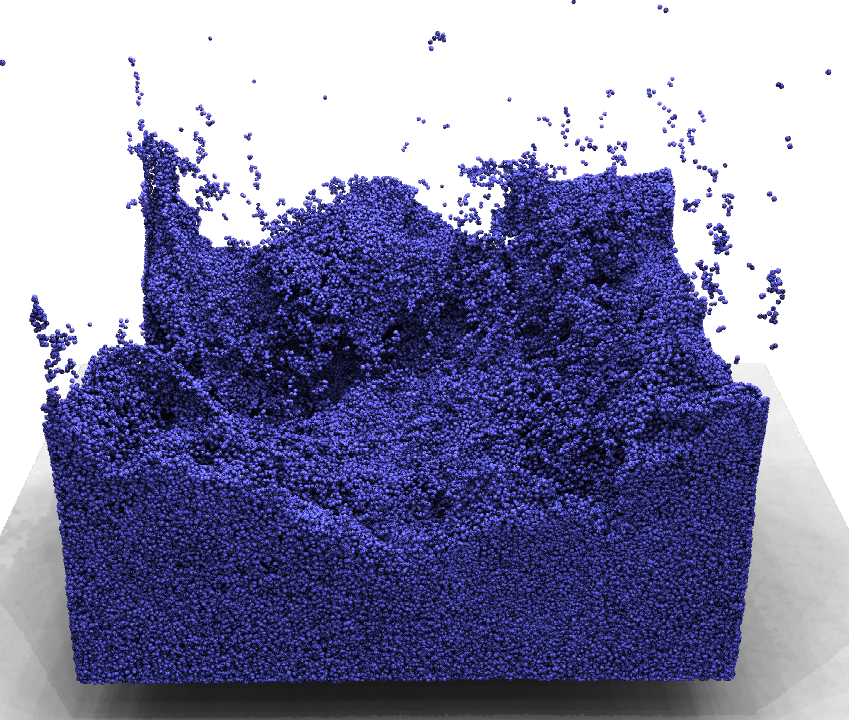
\includegraphics[height=1.5in]{images2/0c.png}
        \label{0}
      \end{center}
    \end{figure}
    
  
    \column{2in}
  
  
    \begin{itemize}
      \item They take the shape of its container.
      \pause
      \item They are not compressible (idealization).
      \pause
      \item Their density is constant. 
      \pause
      \item There is interaction between the particles $\rightarrow$ viscosity, superficial tension.
      
      \end{itemize}
  
    \end{columns}
  
  
  
    \end{frame}

    %%%%%%%%%%%%%%%%%%%%%%%%%%%%%%%%%%%%%%%%%%%%%%%%%%%%%%%%%%%%%%%


\begin{frame}

  \textcolor{mypink1}{Density}

 \vspace{5mm}


   \begin{columns}[c]
   \column{2in}  % slides are 3in high by 5in wide
  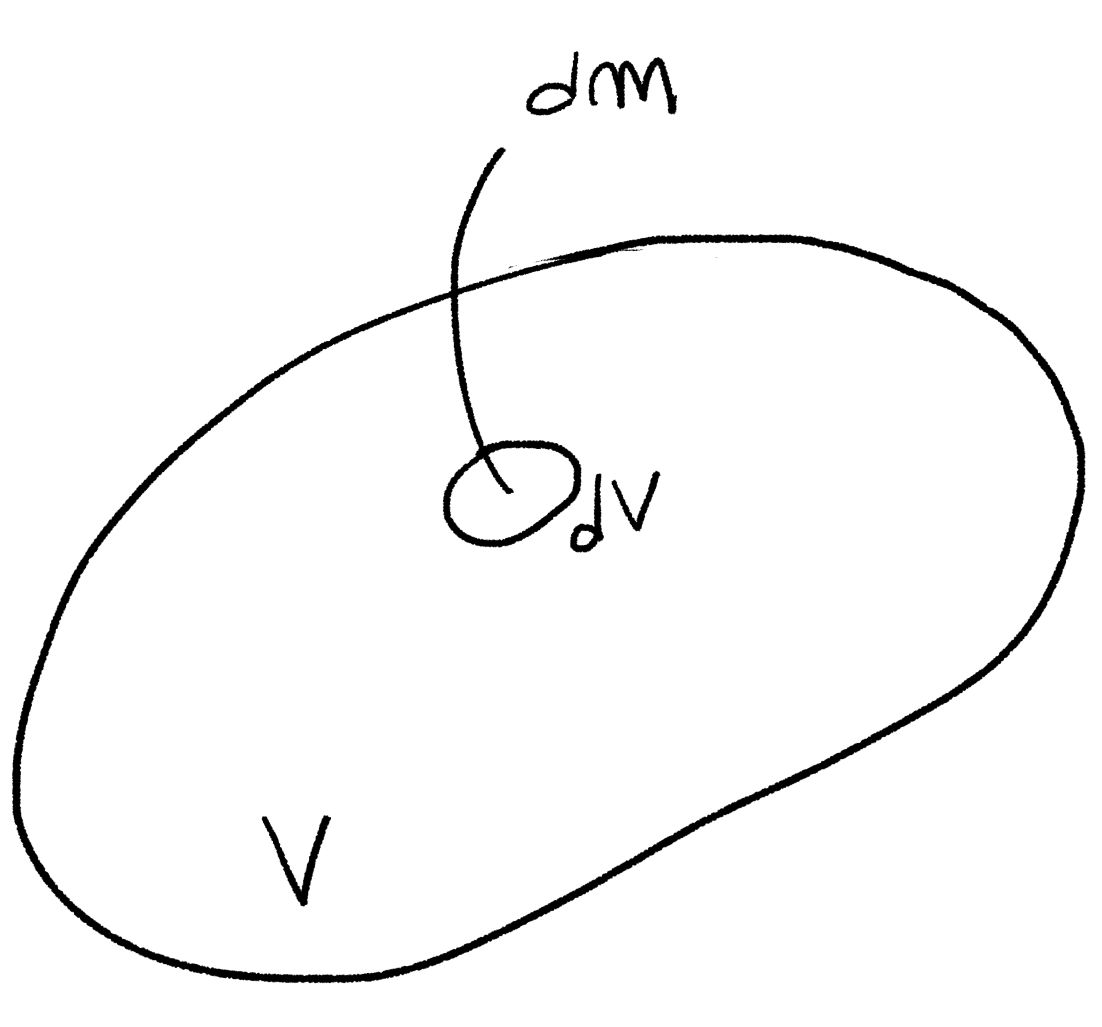
\includegraphics[height=1.7in]{images2/1.jpg}
  
   \column{2in}
    
   \pause
\begin{equation}
\rho=\frac{dm}{dV}
\end{equation}

\pause

\begin{equation*}
\rho=constant \rightarrow \rho =\frac{m}{V}
\end{equation*}

\pause
Then, the weight of an object is,

\pause
\begin{equation*}
w=mg=\rho V g
\end{equation*}


   \end{columns}




  \end{frame}


%%%%%%%%%%%%%%%%%%%%%%%%%%%%%%%%%%%%%%%%%%%%%%%%%%%%%%%%%%%%%%%
\subsection{Pressure}


\begin{frame}

  \textcolor{mypink1}{Pressure}

  \vspace{5mm}
  \pause
  We define the pressure as,
  \pause
  \begin{equation}
  P=\frac{F}{A}
  \end{equation}

  It is an scalar, its units are
  \pause

  \begin{equation}
  [P]=\frac{N}{m^2}=Pa
  \end{equation}
  \vspace{3mm}
  \pause
   At sea level $\rightarrow$ $\boxed{P_0=1.013\times10^5\frac{N}{m^2}=1atm}$

  \vspace{3mm}



  \end{frame}

%%%%%%%%%%%%%%%%%%%%%%%%%%%%%%%%%%%%%%%%%%%%%%%%%%%%%%%%%%%%%%%



\begin{frame}


In a fluid at rest, there are not shear forces, and
\vspace{5mm}

\pause
\begin{itemize}
  \item the pressure is the same in every direction at a given depth
  \pause
  \item the force is perpendicular to any solid surface
\end{itemize}

\vspace{5mm}
\pause
\begin{center}
  \begin{figure}
    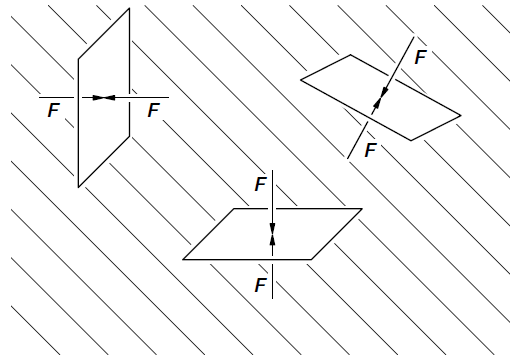
\includegraphics[height=1.7in]{images2/Feiman_1.png}
    \caption[]{Figure from The Feynman Lectures vol II.}
    \label{Feinman_1}
  \end{figure}
\end{center}


  \end{frame}




%%%%%%%%%%%%%%%%%%%%%%%%%%%%%%%%%%%%%%%%%%%%%%%%%%%%%%%%%%%%%%%


\begin{frame}

  \textcolor{mypink1}{The pressure in a static liquid under the force of gravity}

\pause
  \begin{columns}[c]
    \column{2in}  % slides are 3in high by 5in wide
 
      \begin{center}
        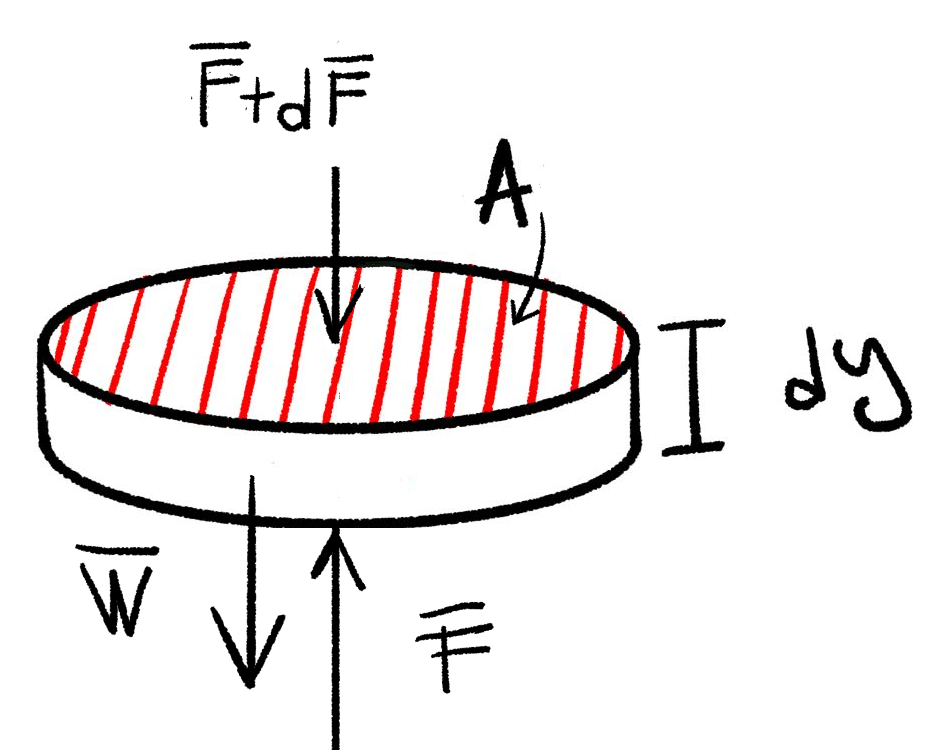
\includegraphics[height=1.3in]{images2/Feiman_2b.png}
      \end{center}

      
\pause

    \column{2.6in}
 
      \begin{equation*}
        Equilibrium \ \rightarrow \sum F_y=0
      \end{equation*}

      \pause
      \begin{equation*}
        \rightarrow F -(F+dF)-W=0
      \end{equation*}

   

\pause

      \begin{equation*}
        \rightarrow PA-(P+dP)A=\rho g A dy
      \end{equation*}

      \pause

      \begin{equation}
        \rightarrow -dP=\rho g  dy 
      \end{equation}
    

    \end{columns}

\end{frame}


  %%%%%%%%%%%%%%%%%%%%%%%%%%%%%%%%%%%%%%%%%%%%%%%%%%%%%%%%%%%%%%%
\begin{frame}

  Then,
  
  \begin{equation*}
  \frac{dP}{dy}=-\rho g 
  \end{equation*}
  
  \vspace{3mm}
  
  $\rightarrow$ The pressure  decreases when y  increases 
  
  \begin{equation*}
  \int^{P_2}_{P_1} dP=- \int^{y_2}_{y_1} \rho g dy
  \end{equation*}
  
  \begin{equation*}
  P_2-P_1=- \int^{y_2}_{y_1} \rho g dy, \ \ \ \rho=\rho(y)
  \end{equation*}
  
    \end{frame}



%%%%%%%%%%%%%%%%%%%%%%%%%%%%%%%%%%%%%%%%%%%%%%%%%%%%%%%%%%%%%%%

\begin{frame}


  \begin{columns}[c]
   \column{2in}  % slides are 3in high by 5in wide
  
  \begin{center}
    \begin{figure}
      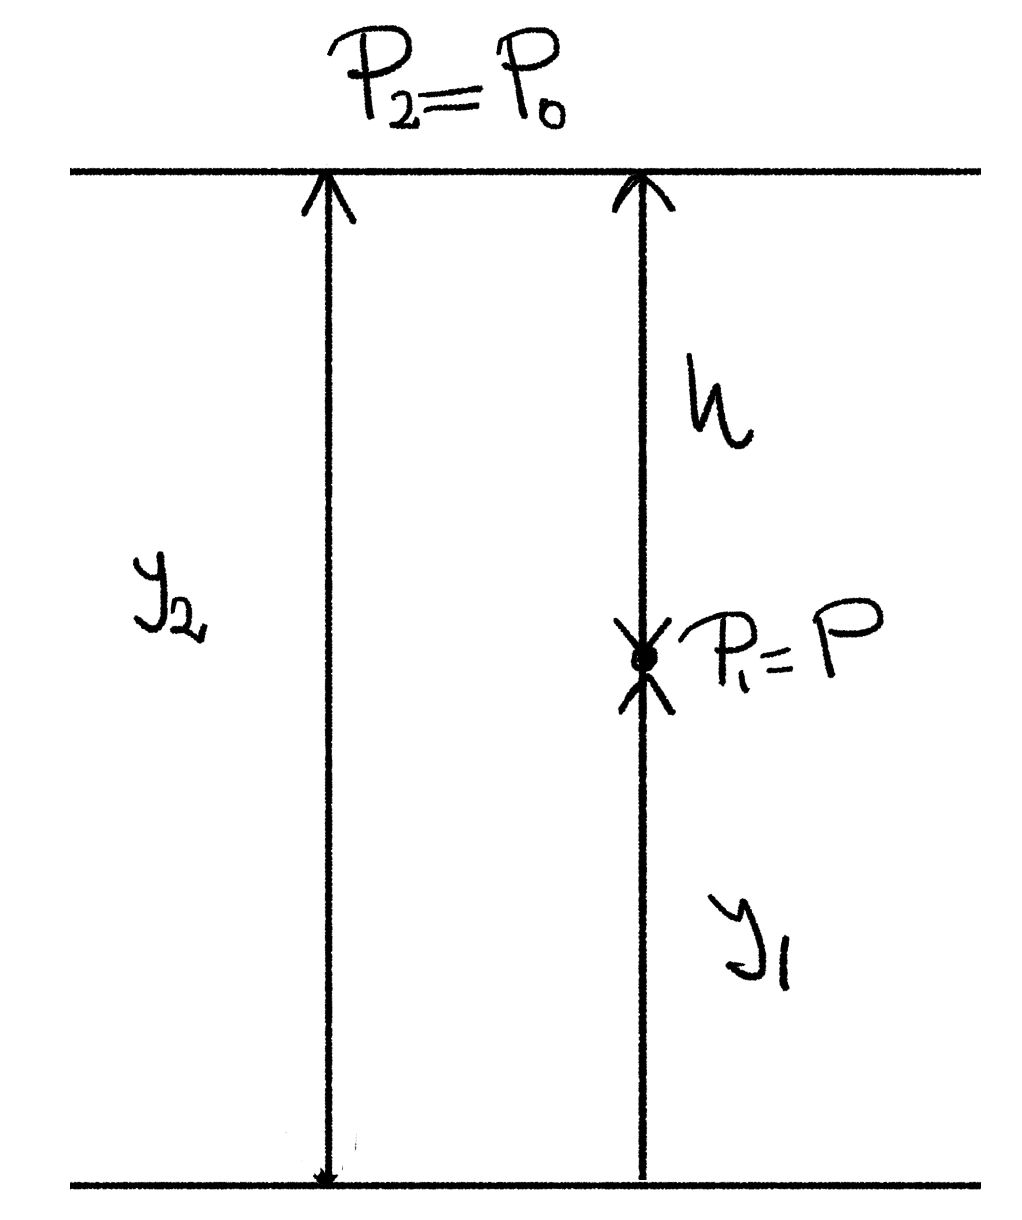
\includegraphics[height=1.7in]{images2/prho3.jpg}
      \caption{$P_0$ is the pressure due to the atmosphere above.}
    \end{figure}

\end{center}


  \column{2in}
    $\rho=constant \rightarrow \Delta P=-\rho g \Delta y$ 

    \begin{equation*}
      P_2-P_1=-\rho g (y_2-y_1)
    \end{equation*}


    \begin{equation*}
      P_0-P=-\rho gh
    \end{equation*}

    \begin{equation}
      \rightarrow  \boxed{P=P_0+\rho gh}
    \end{equation}


   \end{columns}



  \end{frame}

        %%%%%%%%%%%%%%%%%%%%%%%%%%%%%%%%%%%%%%%%%%%%%%%%%%%%%%%%%%%%%%%
        \begin{frame}
          \frametitle{Conceptual Example}
          
              
      
          
          \begin{columns}[c]
            \column{2in}  % slides are 3in high by 5in wide
          
      
            You insert
            a straw of length $\ell$ into a tall glass of water. You place your finger over the
            top of the straw, capturing some air above the water but preventing any additional
            air from getting in or out, and then you lift the straw from the water. You
            find that the straw retains most of the water. 
            \vspace{3mm}
      
       
      
            \column{2in}
        How is $P$? greater than, equal to, or less than the atmospheric pressure $P_0$ outside
          the straw?
                
            \begin{figure}[h!]
              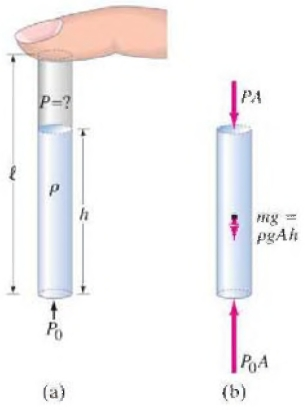
\includegraphics[height=1.5in]{images2/conceptual1.jpg}
          \end{figure} 
      
            \end{columns}
          
          
          
          
          
            \end{frame}
      
%%%%%%%%%%%%%%%%%%%%%%%%%%%%%%%%%%%%%%%%%%%%%%%%%%%%%%%%%%%%%%%
\newcounter{example}
\setcounter{example}{1}

\begin{frame}
\frametitle{Example \theexample }
Pressure at a faucet:  The surface of the water in a storage tank is $30~m$ above a water faucet in the kitchen of a house. Calculate the difference
in water pressure between the faucet and the surface of the water in the tank (density of water:$\rho=10^3~kg/m^3$).

 \begin{center}
  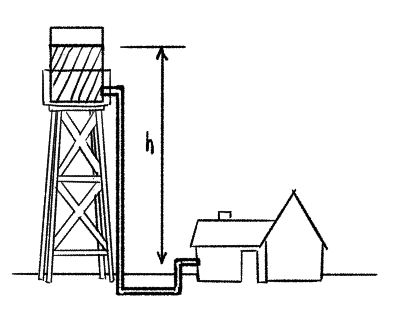
\includegraphics[height=1.7in]{images2/example1.jpg}
\end{center}




  \end{frame}


 %%%%%%%%%%%%%%%%%%%%%%%%%%%%%%%%%%%%%%%%%%%%%%%%%%%%%%%%%%%%%%%


\begin{frame}
\frametitle{Example \theexample }
\textcolor{mypink1}{Solution in whiteboard}




\begin{columns}[c]
  \column{2in}  % slides are 3in high by 5in wide

  \begin{figure}[h!]
    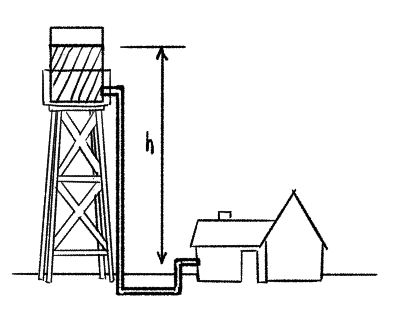
\includegraphics[height=2.4in]{images2/example1.jpg}
\end{figure} 

  \column{2in}


  \end{columns}





  \end{frame}



%%%%%%%%%%%%%%%%%%%%%%%%%%%%%%%%%%%%%%%%%%%%%%%%%%%%%%%%%%%%%%%
\stepcounter{example}

\begin{frame}
\frametitle{Example \theexample}
Force on aquarium window. Calculate the force due to water pressure exerted on a 1.0 m X 3.0 m aquarium viewing window whose top
edge is 1.0 m below the water surface

\vspace{5mm}
\begin{center}
  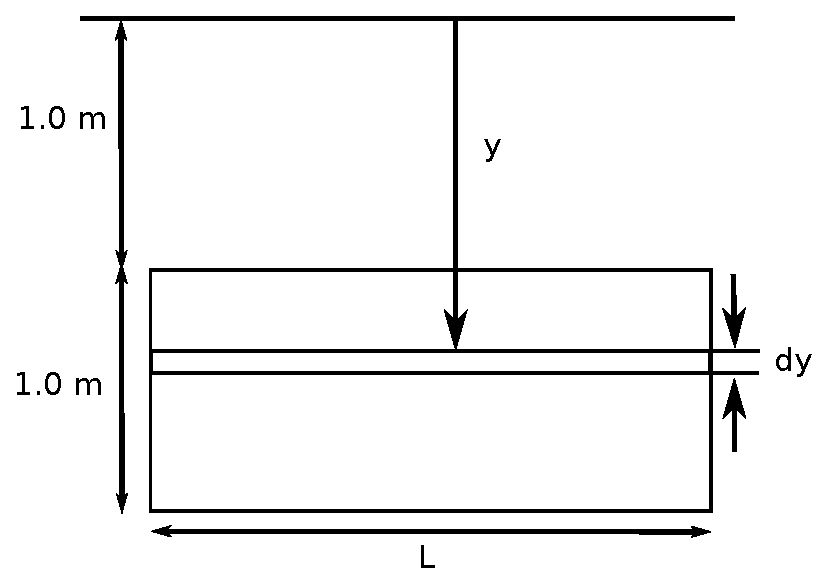
\includegraphics[height=1.4in]{images2/example2.eps}
\end{center}



  \end{frame}

%%%%%%%%%%%%%%%%%%%%%%%%%%%%%%%%%%%%%%%%%%%%%%%%%%%%%%%%%%%%%%%
  \begin{frame}
    \frametitle{Example \theexample }
    \textcolor{mypink1}{Solution in whiteboard}
    
    
    
    
    \begin{columns}[c]
      \column{2in}  % slides are 3in high by 5in wide
    
      \begin{figure}[h!]
        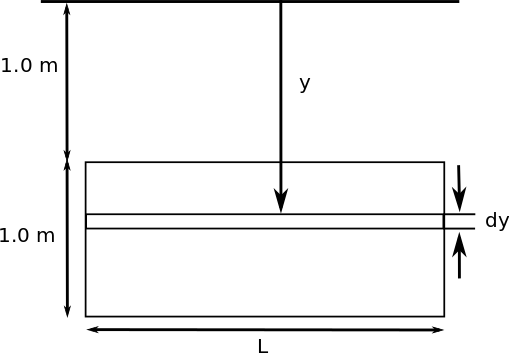
\includegraphics[height=1.5in]{images2/example2.jpg}
    \end{figure} 
    
      \column{2in}
    
    
      \end{columns}
    
    
    
    
    
      \end{frame}



%%%%%%%%%%%%%%%%%%%%%%%%%%%%%%%%%%%%%%%%%%%%%%%%%%%%%%%%%%%%%%%
\begin{frame}
  \frametitle{Atmospheric Pressure}
  What happen if the density is not constant?
  
  \pause
  
  \vspace{3mm}
  
  if we know the relation between $\rho$ and $P$: $ \rho(P)$,
  
  \pause
  
\begin{equation*}
  dP=-g\rho(P)dy 
\end{equation*}


\begin{equation*}
  \rightarrow \frac{dP}{\rho(P)}=-g dy
\end{equation*}


\begin{equation*}
  \rightarrow \int^{P_2}_{P_1} \frac{dP}{\rho(P)}=-g \Delta y
\end{equation*}

  
  \pause
  we can solve the equation and find $P=P(y)$
  \end{frame}
  

%%%%%%%%%%%%%%%%%%%%%%%%%%%%%%%%%%%%%%%%%%%%%%%%%%%%%%%%%%%%%%%
\begin{frame}
\frametitle{Atmospheric Pressure}

\begin{itemize}
  \item Equation of Estate (EoS): relation between $\rho$ and $P$
  \pause
  \vspace{3mm}
  \pause
  \item Ideal gas:  $ \boxed{\rho \propto P}$
\end{itemize}

\pause

\begin{equation*}
  \rightarrow \frac{\rho}{\rho_0}=\frac{P}{P_0}
\end{equation*}
\vspace{3mm}

\pause

 where $\rho_0$ and $P_0$ are the density and pressure at sea level.



  \end{frame}
%%%%%%%%%%%%%%%%%%%%%%%%%%%%%%%%%%%%%%%%%%%%%%%%%%%%%%%%%%%%%%%
\begin{frame}
  \frametitle{Atmospheric Pressure}
  
  \begin{equation*}
    \rightarrow  \frac{dP}{dy}=-\rho g=-\frac{\rho_0P}{P_0}=-P\frac{\rho_0}{P_0}g
  \end{equation*}
  \pause
  \begin{equation*}
  \rightarrow \frac{dP}{P}=-(\frac{\rho_0}{P_0})gdy
  \end{equation*}
  \pause
  \begin{equation*}
  \rightarrow ln(P)-ln(P_0)= ln( \frac{P}{P_0})=-(\frac{\rho_0}{P_0})gy
  \end{equation*}
  
  \pause
  \begin{equation}
  \rightarrow \boxed{P=P_0 e^{-\frac{\rho_0}{P_0}gy}}
  \end{equation}
  
    \end{frame}
%%%%%%%%%%%%%%%%%%%%%%%%%%%%%%%%%%%%%%%%%%%%%%%%%%%%%%%%%%%%%%%
\stepcounter{example}

\begin{frame}
\frametitle{Example \theexample}
At what
elevation is the air pressure equal to half the pressure at sea level?
\pause


\begin{equation*}
  \textcolor{mypink1}{\frac{P_0}{2}=P_0 e^{-\frac{\rho_0}{P_0}gy}}
\end{equation*}
\pause
\begin{equation*}
  \textcolor{mypink1}{\rightarrow ln(\frac{1}{2})=ln( e^{-\frac{\rho_0}{P_0}gy})}
\end{equation*}
\pause
\begin{equation*}
  \textcolor{mypink1}{\rightarrow- ln(2)=-\frac{\rho_0}{P_0}gy}
\end{equation*}
\pause
\begin{equation*}
  \textcolor{mypink1}{\frac{\rho_0}{P_0}g=1.25 \times 10^{-4}m^{-1}}
\end{equation*}
\pause

\begin{equation*}
  \textcolor{mypink1}{\rightarrow\boxed{ y=5550 m}}
\end{equation*}


  \end{frame}


%%%%%%%%%%%%%%%%%%%%%%%%%%%%%%%%%%%%%%%%%%%%%%%%%%%%%%%%%%%%%%%


\begin{frame}
  \textcolor{mypink1}{Spherical geometry: Star Model}
\vspace{3mm}



  
  \begin{center}
  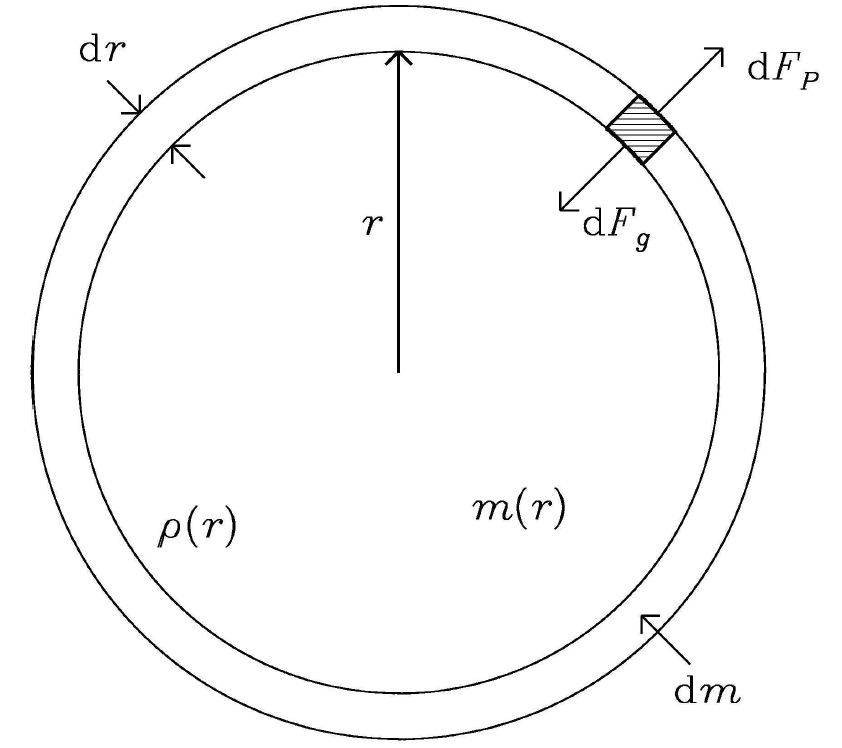
\includegraphics[height=2.in]{images2/star3.jpg}
\end{center}





  \end{frame}




%%%%%%%%%%%%%%%%%%%%%%%%%%%%%%%%%%%%%%%%%%%%%%%%%%%%%%%%%%%%%%%


\begin{frame}


\begin{equation*}
 F_r=PA-(P+dP)A-dF=0
\end{equation*}


  
\begin{equation*}
dF=G\frac{dmM(r)}{r^2}=G\frac{\rho dv M(r)}{r^2}
\end{equation*}

\begin{equation*}
\rightarrow AdP=-G\frac{\rho Adr M(r)}{r^2}
\end{equation*}

\begin{equation}
\rightarrow \boxed{\frac{dP}{dr}=-G\frac{\rho M(r)}{r^2}}
\label{eq:star1}
\end{equation}





  \end{frame}

%%%%%%%%%%%%%%%%%%%%%%%%%%%%%%%%%%%%%%%%%%%%%%%%%%%%%%%%%%%%%%%


\begin{frame}



The equation for the mass is,

\begin{equation}
dM(r)=\rho(r)dV=\rho(r) 4 \pi r^2dr
\end{equation}

\begin{equation}
\rightarrow \frac{dM}{dr}=\rho(r) 4 \pi r^2
\label{eq:star2}
\end{equation}
  
So if we know $\rho(r)$, we can solve the eqs. (\ref{eq:star1}) and (\ref{eq:star2})

  \end{frame}
%%%%%%%%%%%%%%%%%%%%%%%%%%%%%%%%%%%%%%%%%%%%%%%%%%%%%%%%%%%%%%%


% \begin{frame}


  
% Then, we have to solve the system:

% \begin{equation}
%   \left\lbrace
%    \begin{array}{l}
%      \frac{dP}{dr}=-G\frac{\rho M(r)}{r^2}\\
%      \\
%      \frac{dM}{dr}=\rho(r) 4 \pi r^2
%    \end{array}
%    \right.
%    \end{equation}




% With the conditions,




% \begin{equation}
%   \left\lbrace
%    \begin{array}{l}
%     \rho(r=0)=\rho_0\\
%      \\
%      \rho(r=R)=0
%    \end{array}
%    \right.
%    \end{equation}


%   \end{frame}


% %%%%%%%%%%%%%%%%%%%%%%%%%%%%%%%%%%%%%%%%%%%%%%%%%%%%%%%%%%%%%%%


% \begin{frame}


% We need the EoS: $P=P(\rho)$





%   \end{frame}

% %%%%%%%%%%%%%%%%%%%%%%%%%%%%%%%%%%%%%%%%%%%%%%%%%%%%%%%%%%%%%%%


% \begin{frame}


% Then, 

% \begin{itemize}
% \item To model the structure of a Star, we need to find a microscopic model for the matter inside the star (an EoS). 
% \item We need the central density of the star
% \item The mass and Radius of the star depends on the EoS
% \end{itemize}

% \vspace{3mm}

% The pressure is a function of the EoS, and for
% certain conditions it may not be sufficient to withstand the gravitational attraction. Thus
% the structure equations imply there is a maximum mass that a star can have

%   \end{frame}
%%%%%%%%%%%%%%%%%%%%%%%%%%%%%%%%%%%%%%%%%%%%%%%%%%%%%%%%%%%%%%%


\begin{frame}
\frametitle{Pascal's Principle}


If an external pressure $P_0$ is applied to a confined fluid, the pressure at every point 
within the fluid increases by that amount $P_0$.
\vspace{3mm}

 This means that an external pressure acting on a fluid is transmitted throughout the fluid.

\begin{equation}
P=\rho g h+P_0 
\end{equation}


  \end{frame}

%%%%%%%%%%%%%%%%%%%%%%%%%%%%%%%%%%%%%%%%%%%%%%%%%%%%%%%%%%%%%%%


\begin{frame}
\frametitle{Hydrostatic Lift}



 \begin{center}
  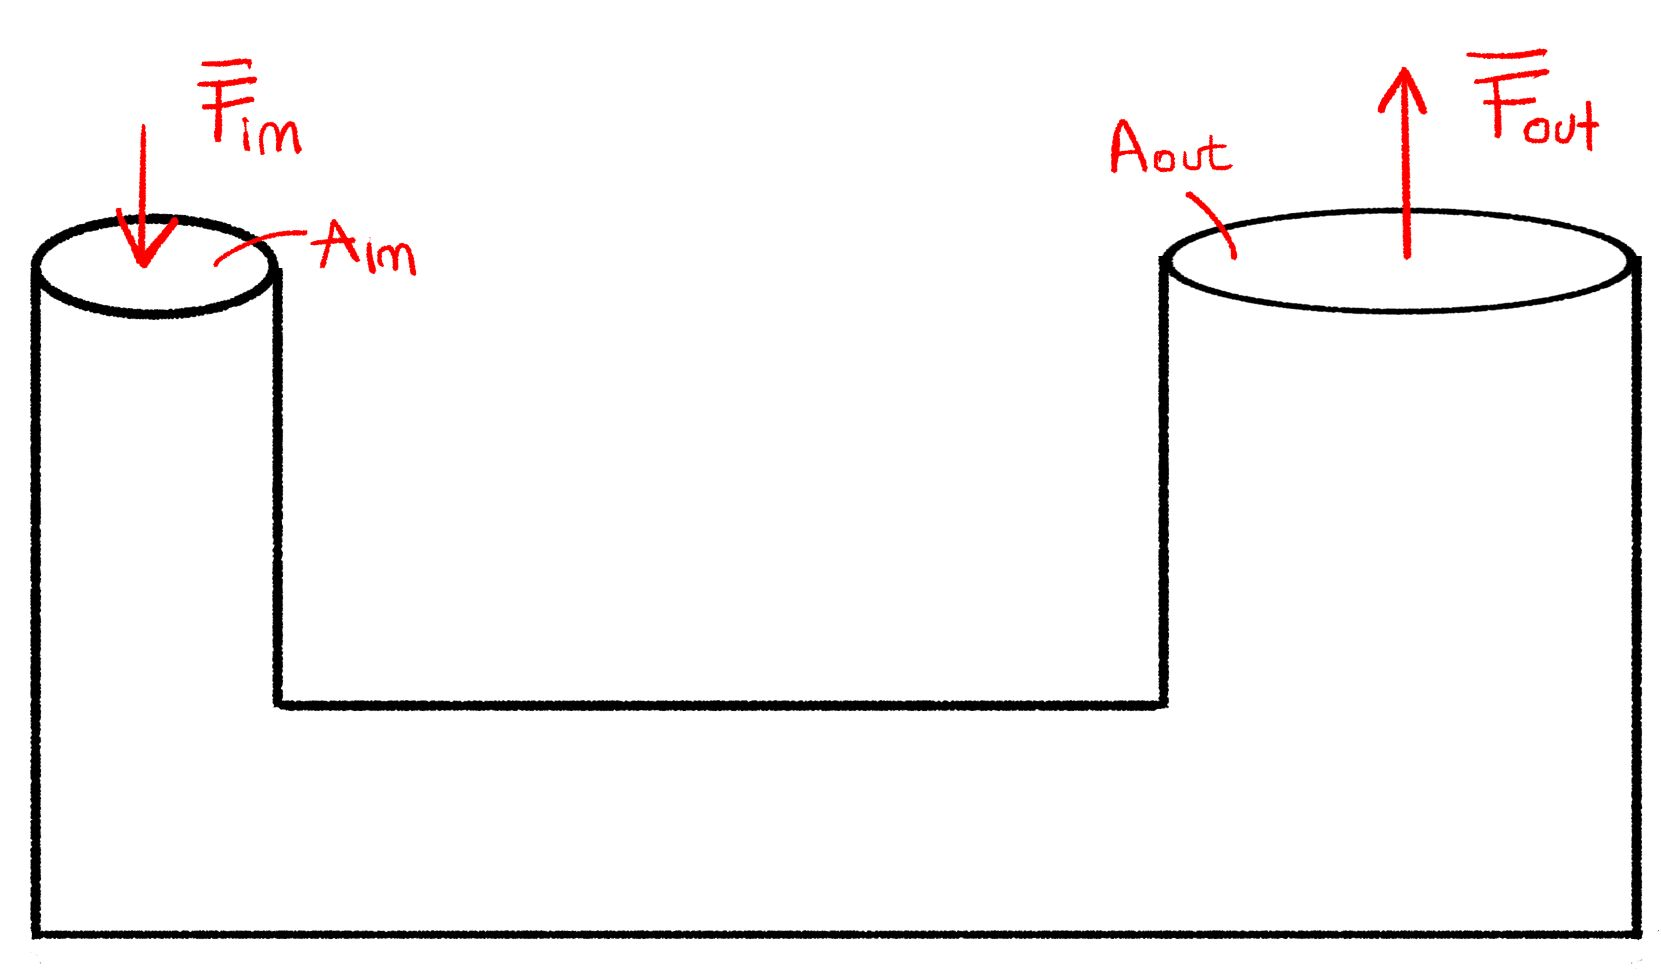
\includegraphics[height=1.3in]{images2/hydrolift.jpg}
\end{center}


\begin{equation}
P_{in}=P_{out} \pause \rightarrow\frac{F_{in}}{A_{in}}=\frac{F_{out}}{A_{out}}
\end{equation}


\begin{equation}
\rightarrow F_{out}=\frac{A_{out}}{A_{in}}F_{in}
\end{equation}


  \end{frame}
%%%%%%%%%%%%%%%%%%%%%%%%%%%%%%%%%%%%%%%%%%%%%%%%%%%%%%%%%%%%%%%

\subsection{Measurement of Pressure}
\begin{frame}
\frametitle{Manometer}

The simplest device to measure the pressure  is the open-tube Manometer,  the Pressure is related to the difference $ \Delta h$ between the two levels of the  liquid.


\begin{equation*}
P=P_0+\rho g \Delta h
\end{equation*} 

  \begin{center}
  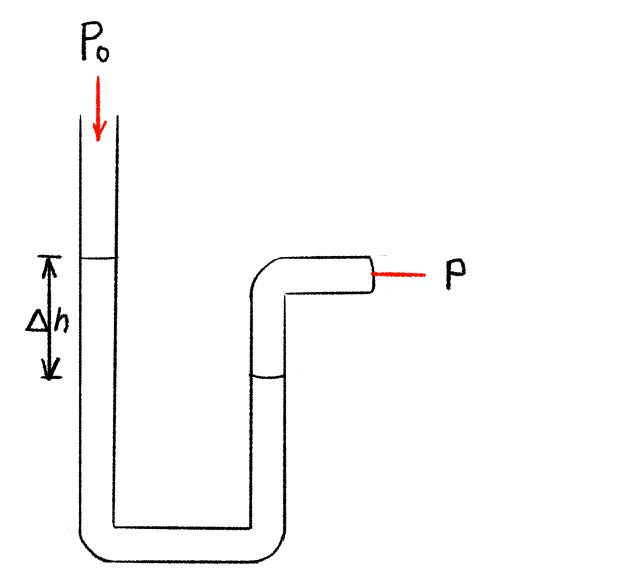
\includegraphics[height=1.7in]{images2/manometer.jpg}
\end{center}


  \end{frame}

%%%%%%%%%%%%%%%%%%%%%%%%%%%%%%%%%%%%%%%%%%%%%%%%%%%%%%%%%%%%%%%

\begin{frame}
\frametitle{Manometer}




Instead of calculating the product $\rho g \Delta h$, sometimes only the change in height $\Delta h$ is specified. In fact, pressures are sometimes specified as so many “millimetres
of mercury” (mm-Hg) or “mm of water” (mm-H20).


  \end{frame}

%%%%%%%%%%%%%%%%%%%%%%%%%%%%%%%%%%%%%%%%%%%%%%%%%%%%%%%%%%%%%%%
\begin{frame}
\frametitle{Barometer}

A barometer is a glass tube completely filled with mercury and then inverted into a bowl of mercury. If the tube is long enough, the level of the mercury will drop, leaving a
vacuum at the top of the tube.

   \begin{columns}[c]
   \column{2in}  % slides are 3in high by 5in wide
    \begin{center}
  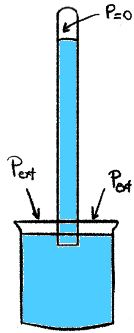
\includegraphics[height=1.8in]{images2/Barometer.jpg}
\end{center}

   \column{2in}
\begin{equation*}
P_{ext}=\rho g \Delta h +0
\end{equation*}
   \end{columns}




  \end{frame}

%%%%%%%%%%%%%%%%%%%%%%%%%%%%%%%%%%%%%%%%%%%%%%%%%%%%%%%%%%%%%%%


\begin{frame}
\frametitle{Barometer}


When $P_{ext}=P_0$, $\Delta h=0.76 cm$. That is, the atmospheric pressure can support a column of mercury only about 76 cm high.

\vspace{3mm}

If we replace the liquid by water, the column high would be $\sim 10 m$

  \end{frame}
%%%%%%%%%%%%%%%%%%%%%%%%%%%%%%%%%%%%%%%%%%%%%%%%%%%%%%%%%%%%%%%
  \stepcounter{example}

  \begin{frame}
  \frametitle{Example \theexample}
  

  A U-shaped
  tube with a horizontal portion of
  length $\ell$ contains
  a liquid. What is the difference
  in height between the liquid
  columns in the vertical arms (a)
  if the tube has an acceleration a
  toward the right and (b) if the
  tube is mounted on a horizontal
  turntable rotating with an angular speed $\omega$with one of the vertical
  arms on the axis of rotation? (c) Explain why the difference in
  height does not depend on the density of the liquid or on the crosssectional
  area of the tube. Would it be the same if the vertical tubes
  did not have equal cross-sectional areas? Would it be the same if the
  horizontal portion were tapered from one end to the other? Explain.

  
 


    \end{frame}

    %%%%%%%%%%%%%%%%%%%%%%%%%%%%%%%%%%%%%%%%%%%%%%%%%%%%%%%%%%%%%%%

    \begin{frame}
    \frametitle{Example \theexample}
    
  

    
    \begin{center}
      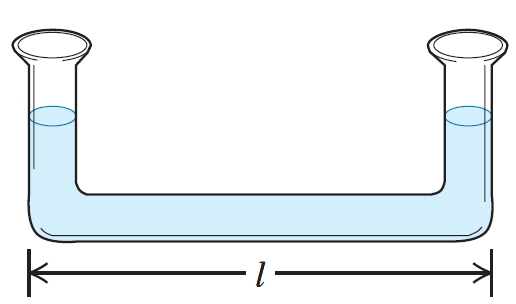
\includegraphics[height=1.6in]{images2/example_12.85.jpg}
    \end{center}
  
  
  
  
      \end{frame}

%%%%%%%%%%%%%%%%%%%%%%%%%%%%%%%%%%%%%%%%%%%%%%%%%%%%%%%%%%%%%%%
\subsection{Buoyancy}

\begin{frame}
  \textcolor{mypink1}{Archimedes' Principle}

  \vspace{5mm}
Consider a cylinder immersed in a liquid, the upward force exerted by the liquid is the \textbf{Buoyant Force}

\vspace{5mm}

\begin{columns}[c]
  \column{2in}  % slides are 3in high by 5in wide
    \begin{center}
  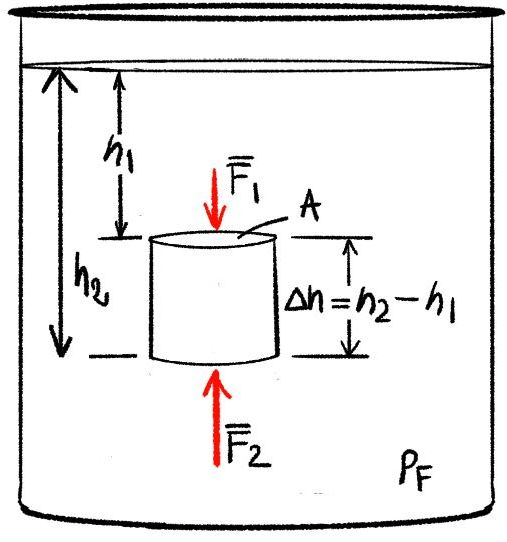
\includegraphics[height=1.6in]{images2/Buoyance.jpg}
\end{center}

  \column{2in}
    \begin{eqnarray*}
      F_B&=&F_2-F_1\\
      &=&\rho_F g A (h_2-h_1)\\
      &=&\rho_F g A \Delta h\\
      &=&m_f g
    \end{eqnarray*}
  \end{columns}
\end{frame}

    
%%%%%%%%%%%%%%%%%%%%%%%%%%%%%%%%%%%%%%%%%%%%%%%%%%%%%%%%%%%%%%%


\begin{frame}
\frametitle{Archimedes' Principle in general }
For any irregular body...

  \begin{figure}
    \begin{center}
      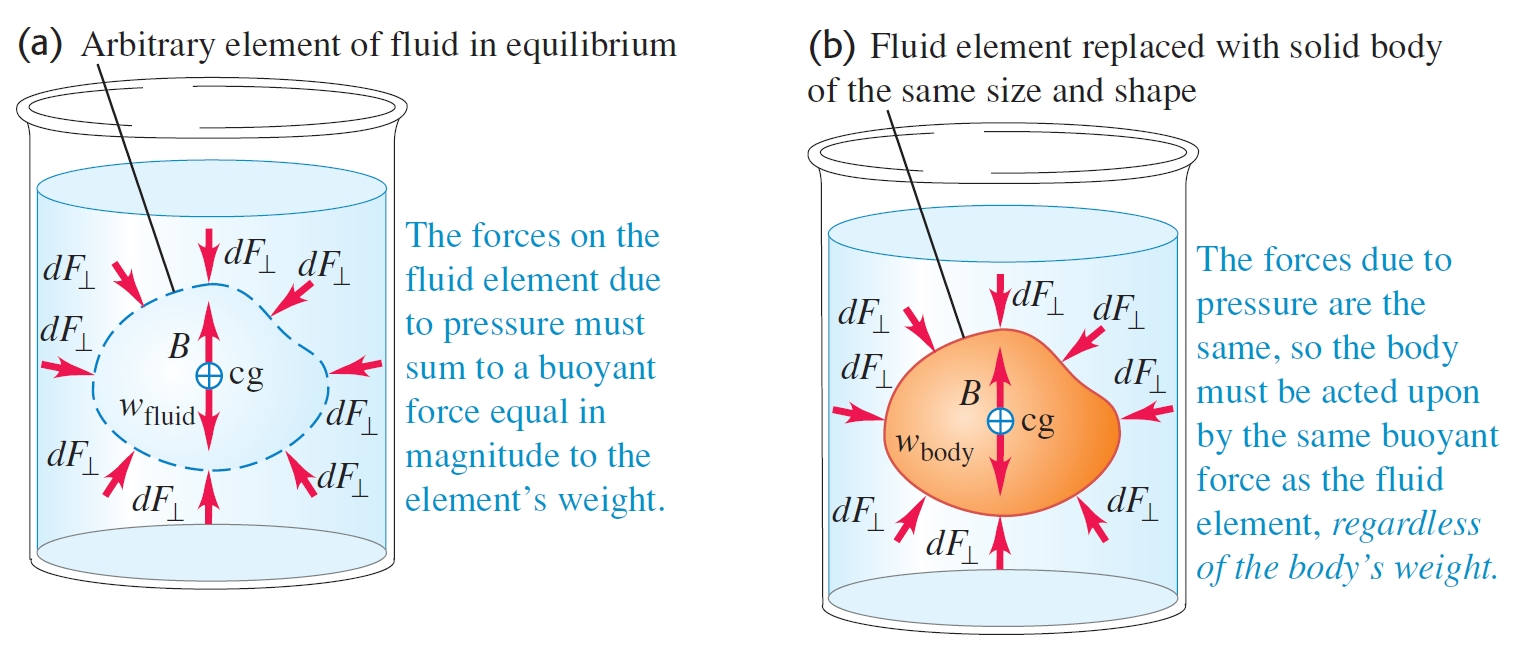
\includegraphics[height=1.8in]{images2/Buoyance2b.jpg}
    \end{center}
    \caption{Figure from sears and zemansky's university physics 13th edition volume 1.}
  \end{figure}


  \end{frame}

%%%%%%%%%%%%%%%%%%%%%%%%%%%%%%%%%%%%%%%%%%%%%%%%%%%%%%%%%%%%%%%

\begin{frame}

    
  
  \textit{\textcolor{mypink1}{The buoyant force on an object immersed in
   a fluid is equal to the weight of the fluid displaced by that object.}}
    
    
\end{frame}


%%%%%%%%%%%%%%%%%%%%%%%%%%%%%%%%%%%%%%%%%%%%%%%%%%%%%%%%%%%%%%%


\begin{frame}
\textbf{Two pails of water}. Consider two identical pails of water filled to the brim. One pail contains only water, the other has a piece of wood floating in it. Which pail has the greater weight?

\vspace{3mm}

\pause
\textcolor{mypink1}{\textbf{Answer}  Both pails weigh the same. Recall Archimedes’ principle: the wood
displaces a volume of water with weight equal to the weight of the wood.
Some water will overflow the pail, but Archimedes’ principle tells us the
spilled water has weight equal to the weight of the wood object; so the pails have
the same weight.}
  \end{frame}

%%%%%%%%%%%%%%%%%%%%%%%%%%%%%%%%%%%%%%%%%%%%%%%%%%%%%%%%%%%%%%%



\begin{frame}


\textbf{Object in equilibrium} 

\vspace{3mm}
The object is in equilibrium when


   \begin{eqnarray*}
    m_Fg&=&m_og\\
    \pause
    \rightarrow \rho_FV_{dis}g&=&\rho_OV_Og\\
    \pause
    \rightarrow \frac{V_{dis}}{V_{O}}&=&\frac{ \rho_O}{\rho_{F } }
    \end{eqnarray*}
    
    Where $V_{dis}/V_{O}$ is  the fraction of submerged Vol.
    

  \end{frame}
  %%%%%%%%%%%%%%%%%%%%%%%%%%%%%%%%%%%%%%%%%%%%%%%%%%%%%%%%%%%%%%%



 \begin{frame}


   \textbf{Object in equilibrium} 
  
   \vspace{3mm}
  
   \begin{columns}[c]
      \column{2in}  % slides are 3in high by 5in wide
  
      \begin{center}
     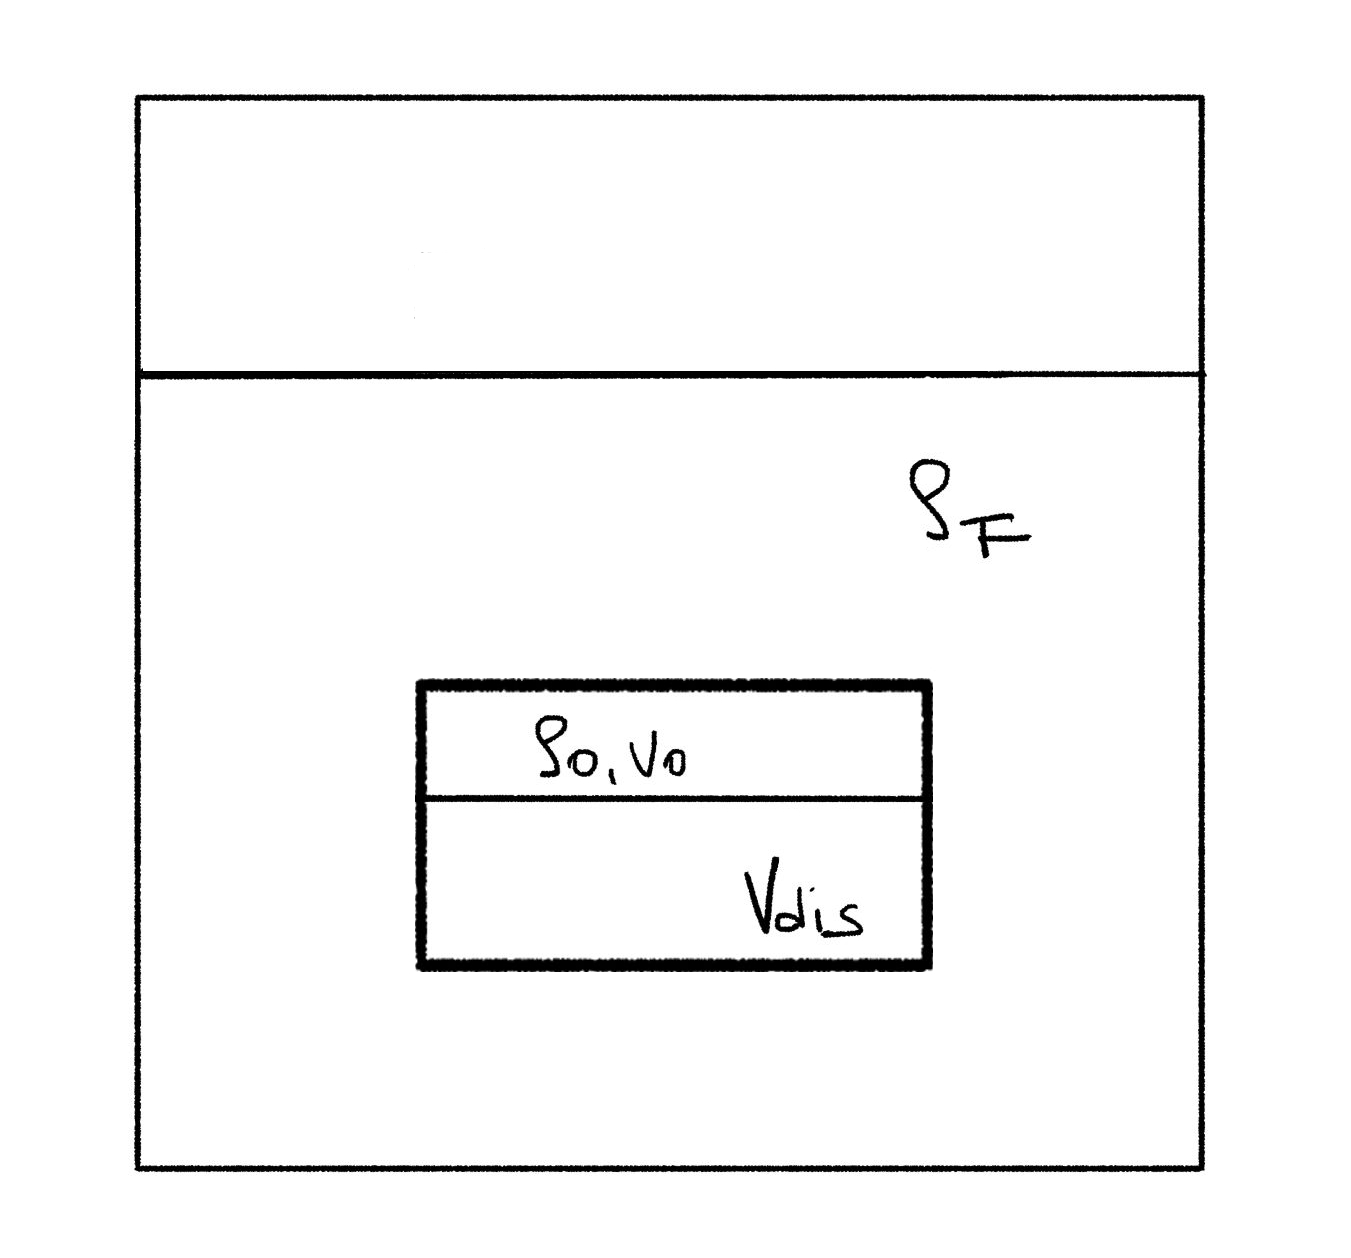
\includegraphics[height=1.7in]{images2/Buoyance3b.jpg}
   \end{center}
   
      \column{2in}
  
   
      If   $\rho_O/\rho_{F }=1\pause\rightarrow V_o=V_{disp}$ 

      \pause

      \vspace{3mm}

      Then, the object is completely submerged and in equilibrium

      \end{columns}
  
  
  
     \end{frame}
%%%%%%%%%%%%%%%%%%%%%%%%%%%%%%%%%%%%%%%%%%%%%%%%%%%%%%%%%%%%%%%



\begin{frame}


\textbf{Floating objects} 

\vspace{3mm}



\begin{columns}[c]
   \column{2in}  % slides are 3in high by 5in wide

   \begin{center}
  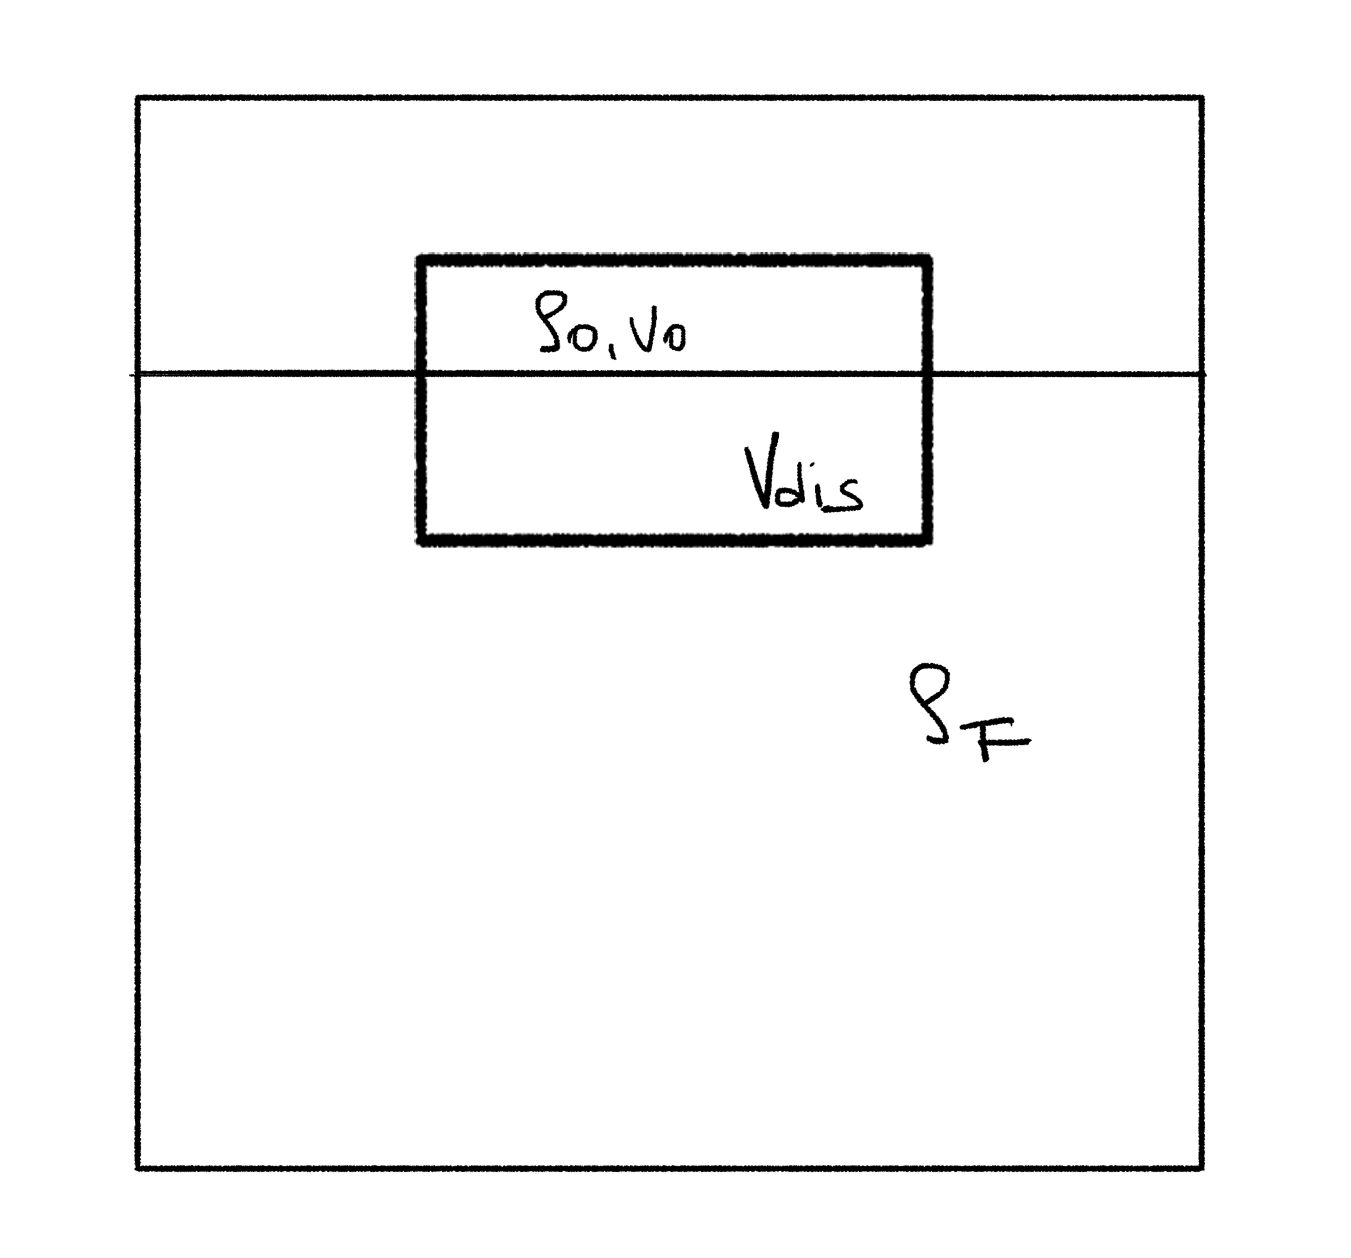
\includegraphics[height=1.7in]{images2/Buoyance3.jpg}
\end{center}
 
   \column{2in}

   If   $\rho_O/\rho_{F }<1\pause\rightarrow V_o>V_{disp}$ 

   \pause

   \vspace{3mm}
   Then, the object floats

   \end{columns}



  \end{frame}

  %%%%%%%%%%%%%%%%%%%%%%%%%%%%%%%%%%%%%%%%%%%%%%%%%%%%%%%%%%%%%%%



\begin{frame}


\textbf{Sank object} 

\vspace{3mm}
In this case, $F_B<mg$, then, the object is in equilibrium when


\begin{columns}[c]
   \column{2in}  % slides are 3in high by 5in wide

   \begin{center}
  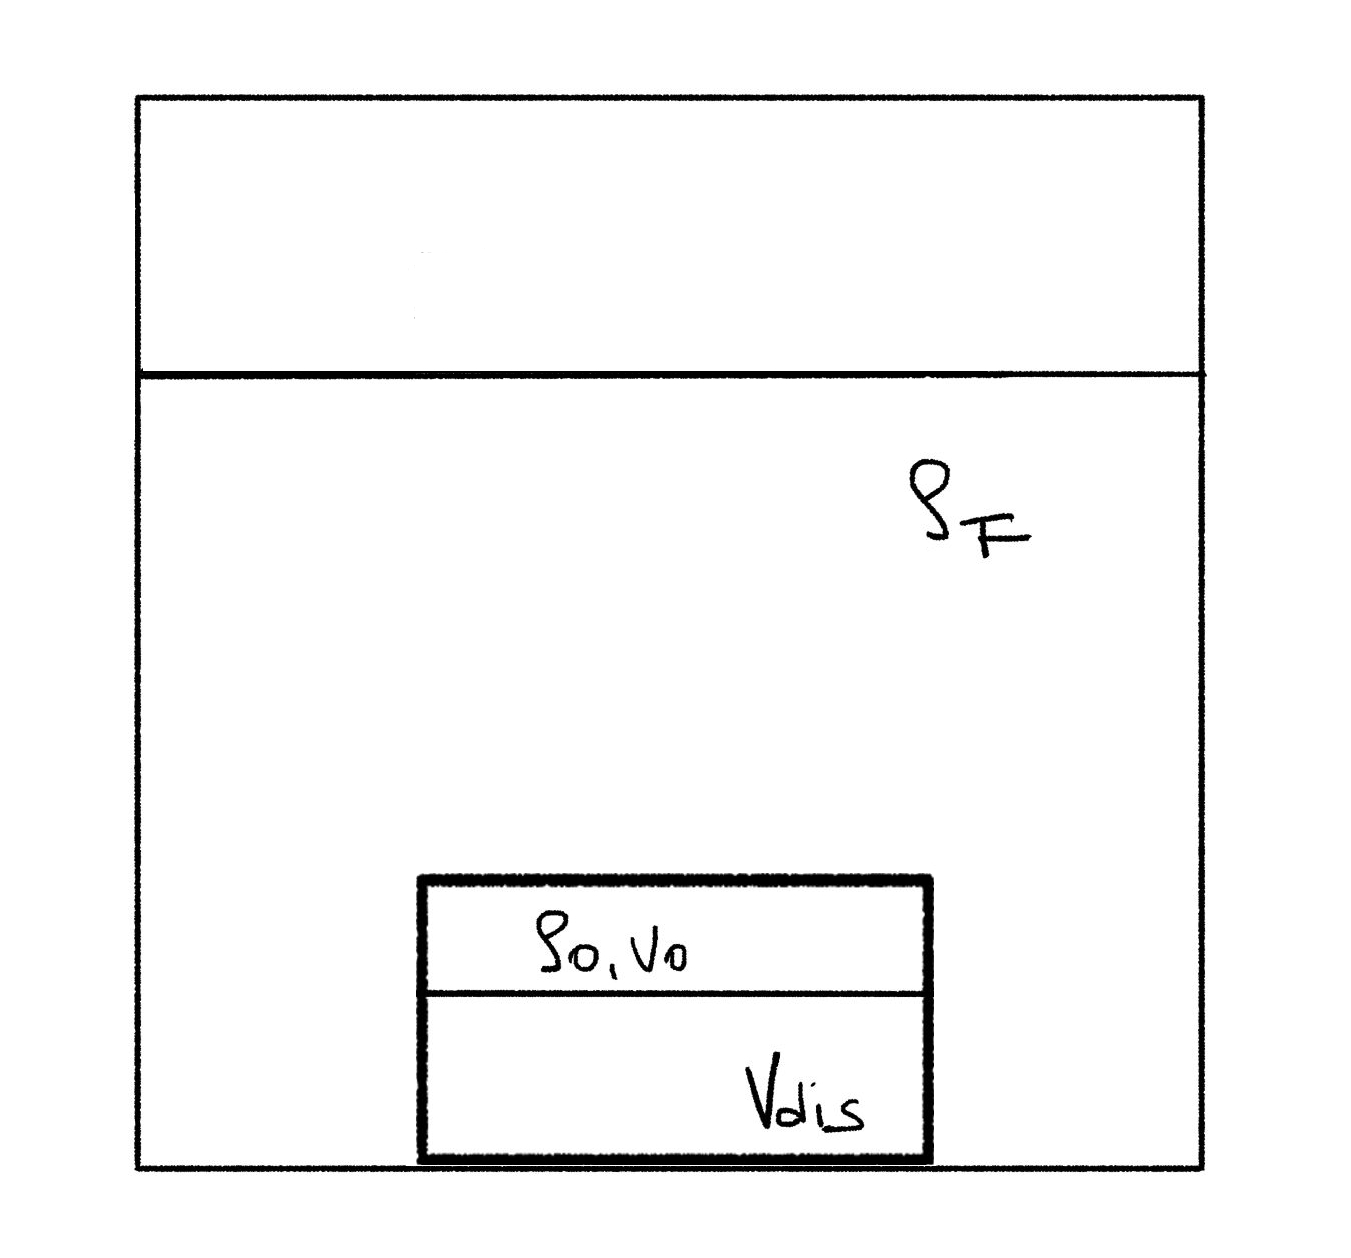
\includegraphics[height=1.7in]{images2/Buoyance3c.jpg}
\end{center}
 
   \column{2in}



   If   $\rho_O/\rho_{F }>1\pause\rightarrow no ~equilibrium$ 
   
   \pause

   \vspace{3mm}
   
   The, the object sinks.


  


   \end{columns}



  \end{frame}
%%%%%%%%%%%%%%%%%%%%%%%%%%%%%%%%%%%%%%%%%%%%%%%%%%%%%%%%%%%%%%%

\stepcounter{example}

\begin{frame}
\frametitle{Example \theexample}

\textbf{Recovering a submerged statue}. A 70-kg ancient statue lies at the bottom of the sea. Its volume is $3.0 \times 10^4cm^3$. How much force is
needed to lift it?

  \end{frame}
%%%%%%%%%%%%%%%%%%%%%%%%%%%%%%%%%%%%%%%%%%%%%%%%%%%%%%%%%%%%%%%
\begin{frame}
  
\stepcounter{example}

\frametitle{Example \theexample}

\textbf{Archimedes:} Is the crown gold? When a crown of mass $14.7~kg$
is submerged in water, an accurate scale reads only $13.4~kg$. Is the crown made of gold?

  \begin{center}
  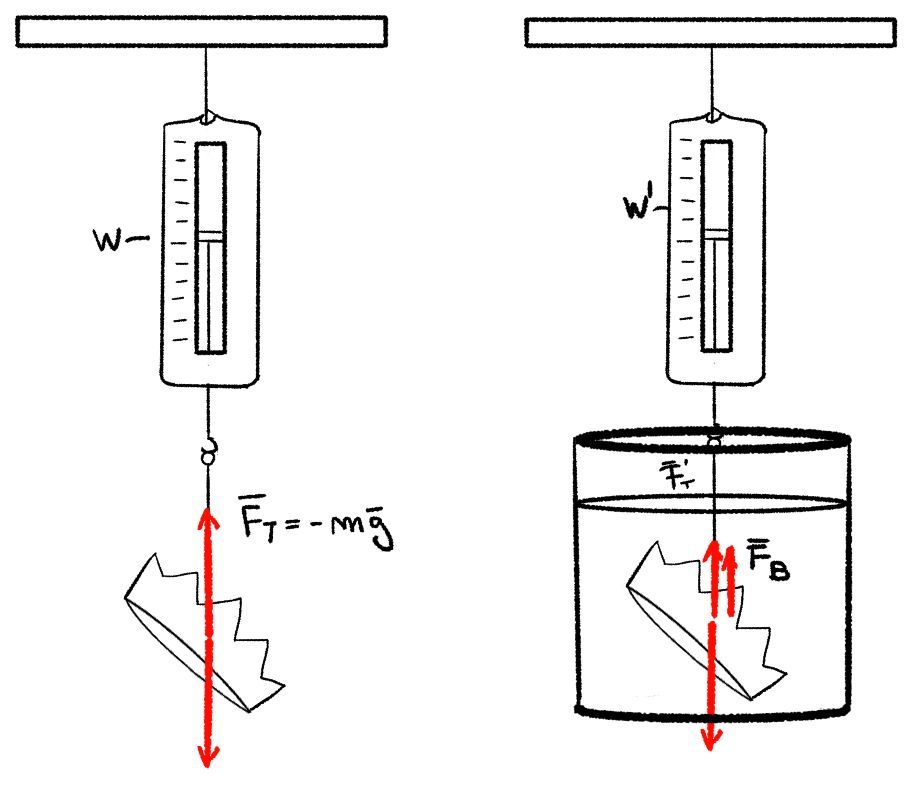
\includegraphics[height=1.7in]{images2/arquimedes.jpg}
\end{center}

  \end{frame}



%%%%%%%%%%%%%%%%%%%%%%%%%%%%%%%%%%%%%%%%%%%%%%%%%%%%%%%%%%%%%%%

\stepcounter{example}
\begin{frame}
\frametitle{Example \theexample}

Helium balloon. What volume V of helium is needed if a balloon is to lift a load of $180~kg$ (including the weight of the empty balloon)?


  \begin{center}
  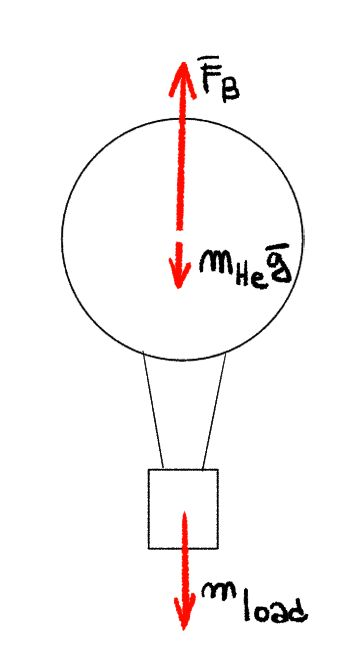
\includegraphics[height=2.in]{images2/baloom.jpg}
\end{center}

  \end{frame}
%%%%%%%%%%%%%%%%%%%%%%%%%%%%%%%%%%%%%%%%%%%%%%%%%%%%%%%%%%%%%%%


\stepcounter{example}
\begin{frame}
\frametitle{Example \theexample}


Suppose a piece of styrofoam, $\rho=180~kg/m^3$ is
held completely submerged in water. (a) What is the
tension in the cord? Find this using Archimedes’s principle.
(b) Use $p=p_0+\rho g h$ to calculate directly the force exerted by
the water on the two sloped sides and the bottom of the styrofoam;
then show that the vector sum of these forces is the buoyant
force.

  \begin{center}
  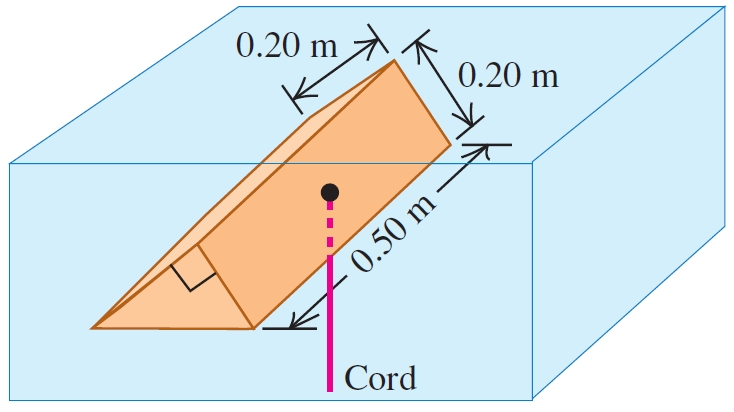
\includegraphics[height=1.5in]{images2/example_12.97.jpg}
\end{center}

  \end{frame}

  %%%%%%%%%%%%%%%%%%%%%%%%%%%%%%%%%%%%%%%%%%%%%%%%%%%%%%%%%%%%%%%

\begin{frame}
\frametitle{Example \theexample}







\begin{columns}[c]
  \column{2in}  % slides are 3in high by 5in wide

  \begin{center}
    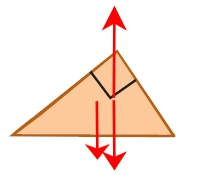
\includegraphics[height=1.2in]{images2/example_12.97b.jpg}
  \end{center}
  

  \column{2in}
  
  a)
  \textcolor{mypink1}{
  \begin{eqnarray*}
   F_B-T-W&=&0\\
   \pause
   \rightarrow T&=&(\rho_w -\rho_o) V g\\
   \pause
   \rightarrow T&=&\frac{1}{2}a^2\ell(\rho_w -\rho_o)g\\
  \end{eqnarray*}
  }
  \end{columns}





  \end{frame}


  %%%%%%%%%%%%%%%%%%%%%%%%%%%%%%%%%%%%%%%%%%%%%%%%%%%%%%%%%%%%%%%

  \begin{frame}
    \frametitle{Example \theexample}
    
   
    
    \begin{columns}[c]
      \column{1.in}  % slides are 3in high by 5in wide
    
      \begin{center}
        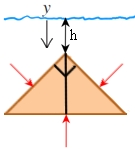
\includegraphics[height=1.2in]{images2/example_12.97c.jpg}
      \end{center}
      
    
      \column{2.5in}
      
      b) sides:
      \textcolor{mypink1}{
      \begin{eqnarray*}
      dF&=&PdA\\
       \pause
      dA &=&\ell dr\\
      \pause
      &=&\ell\frac{2}{\sqrt{2}}dy\\
      \pause
      \rightarrow dF&=&\frac{2}{\sqrt{2}}\rho g y\ell dy\\
      \pause
      \rightarrow F&=&\frac{2}{\sqrt{2}} \ell \rho g \int^{h+\sqrt{2}/2 a}_{h} y dy\\
      \pause
      &=&\boxed{\rho g a h \ell + \frac{\rho g}{2\sqrt{2}}a^2\ell}\\
      \end{eqnarray*}
      }
      \end{columns}
    
      
    
      \end{frame}


        %%%%%%%%%%%%%%%%%%%%%%%%%%%%%%%%%%%%%%%%%%%%%%%%%%%%%%%%%%%%%%%

  \begin{frame}
    \frametitle{Example \theexample}
    
   
    
    \begin{columns}[c]
      \column{1.in}  % slides are 3in high by 5in wide
    
      \begin{center}
        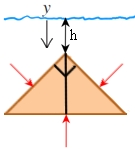
\includegraphics[height=1.2in]{images2/example_12.97c.jpg}
      \end{center}
      
    
      \column{2.5in}
      
      b) bottom:
      \textcolor{mypink1}{
      \begin{eqnarray*}
      F_{Bo}&=&\rho g (h+\frac{\sqrt{2}}{2}a)a \sqrt{2} \ell\\
      \end{eqnarray*}
      }
      \end{columns}
    
      
    
      \end{frame}

        %%%%%%%%%%%%%%%%%%%%%%%%%%%%%%%%%%%%%%%%%%%%%%%%%%%%%%%%%%%%%%%

        \begin{frame}
          \frametitle{Example \theexample}
          
         
          
          \begin{columns}[c]
            \column{1.in}  % slides are 3in high by 5in wide
          
            \begin{center}
              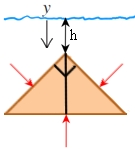
\includegraphics[height=1.2in]{images2/example_12.97c.jpg}
            \end{center}
            
          
            \column{2.5in}
            
             Total:
            \textcolor{mypink1}{
            \begin{eqnarray*}
            F_B&=&F_{Bo}-2F_S\frac{\sqrt{2}}{2}\\
            \pause
            &=&\rho g \frac{a^2 \ell}{2}\\
            \pause
            &=&\rho g V\\
            \pause
            &=&\boxed{g m_w} \ \ \checkmark\\
            \end{eqnarray*}
            }
            \end{columns}

            \end{frame}
%%%%%%%%%%%%%%%%%%%%%%%%%%%%%%%%%%%%%%%%%%%%%%%%%%%%%%%%%%%%%%%


\begin{frame}
  \textcolor{mypink1}{Generalization}
  \vspace{5mm}

\begin{itemize}
\item The pressure on any object is perpendicular to the surface.
\item If the only external force is the gravity, near earth, we have $\frac{dP}{dy}=-\rho g$
\item The Arquimede's Principle is a consequence of the previous 2 items. 
\end{itemize}


  \end{frame}
%%%%%%%%%%%%%%%%%%%%%%%%%%%%%%%%%%%%%%%%%%%%%%%%%%%%%%%%%%%%%%%
\begin{frame}
  \textcolor{mypink1}{Generalization}
  \vspace{5mm}



If the external force is the gravity,

\vspace{3mm}

\begin{equation*}
\frac{dP}{dy}=-\rho g 
\end{equation*}

\pause

\vspace{3mm}

Which is the equivalent expression for an arbitrary force?
\vspace{3mm}

\pause
In general,
\vspace{3mm}

\begin{equation}
\vec{F}=\vec{F}(x,y,z), \ \ P=P(x,y,z)
\end{equation}

  \end{frame}
%%%%%%%%%%%%%%%%%%%%%%%%%%%%%%%%%%%%%%%%%%%%%%%%%%%%%%%%%%%%%%%

\begin{frame}
  \textcolor{mypink1}{Generalization}
  \vspace{5mm}

The resultant force on the x-direction due to the pressure of the liquid is,


 \begin{center}
  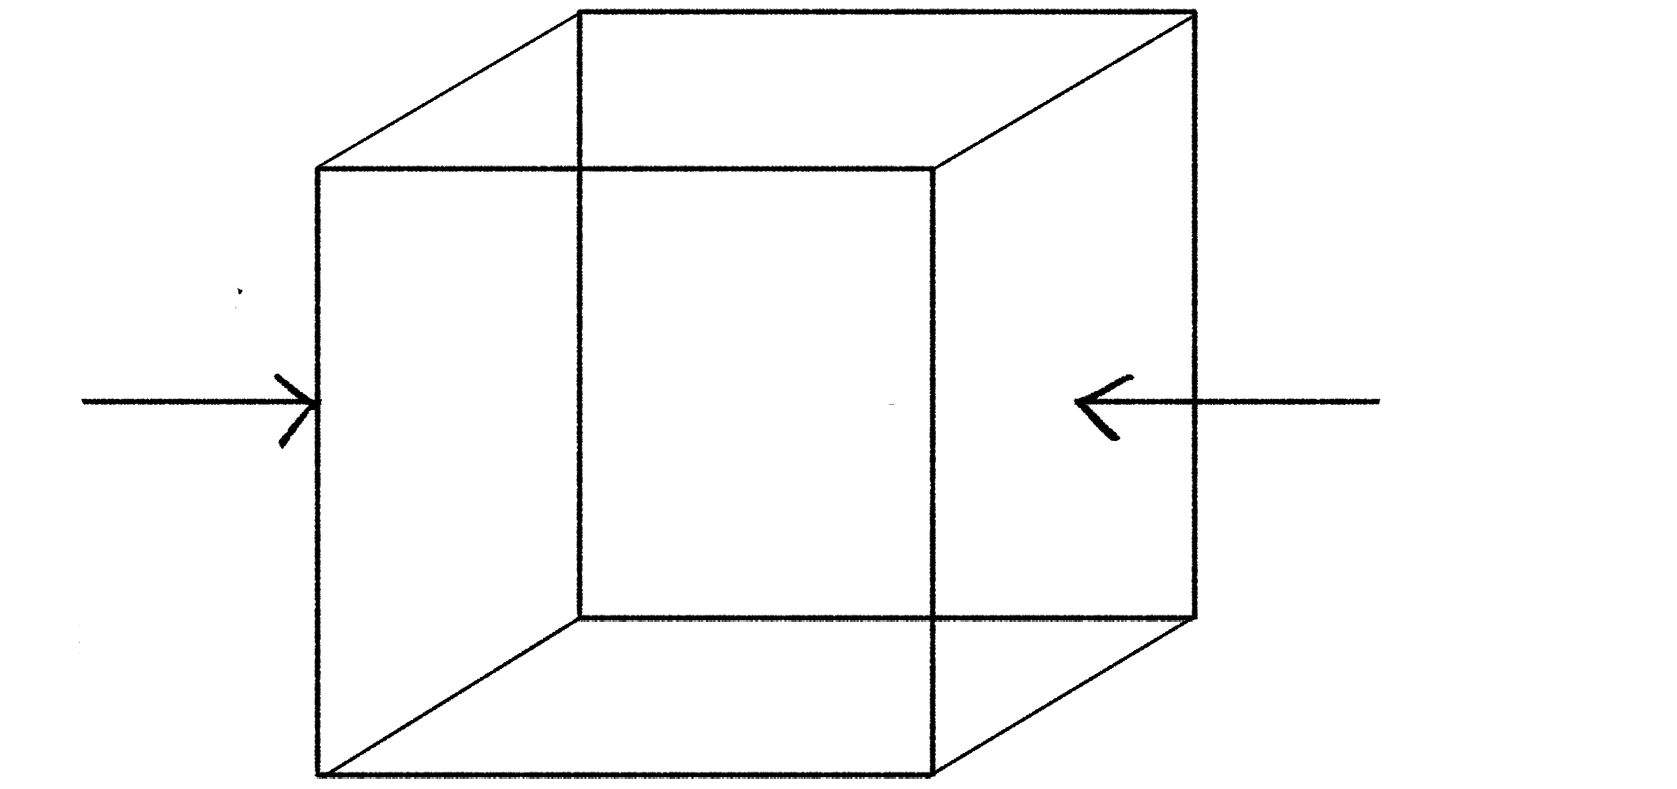
\includegraphics[height=1.in]{images2/generalization1.jpg}
\end{center}

\pause
\begin{equation*}
F_x=Pdydz-(P+dP_x)dydz=-dP_xdydz
\end{equation*}

\pause

and, 

\begin{equation*}
dP_x=\frac{\partial P}{\partial x}dx
\end{equation*}




  \end{frame}

%%%%%%%%%%%%%%%%%%%%%%%%%%%%%%%%%%%%%%%%%%%%%%%%%%%%%%%%%%%%%%%



\begin{frame}
  \textcolor{mypink1}{Generalization}
  \vspace{5mm}

Then, 

\begin{equation*}
F_x=-\frac{\partial P}{\partial x}dxdydz
\end{equation*}

or,


\begin{equation*}
f_x=-\frac{\partial P}{\partial x}
\end{equation*}

where $f_x$ is the force per unit volume.
\vspace{3mm}

\pause

The fluid is in hydrostatic equilibrium if,


\begin{equation*}
f_x+f^{e}_x=0
\end{equation*}



  \end{frame}



%%%%%%%%%%%%%%%%%%%%%%%%%%%%%%%%%%%%%%%%%%%%%%%%%%%%%%%%%%%%%%%

\begin{frame}
  \textcolor{mypink1}{Generalization}
  \vspace{5mm}

Then,

\begin{equation*}
-\frac{\partial P}{\partial x}=-f^{e}_x
\end{equation*}



\pause

If the external force is conservative,

\begin{equation*}
f^e_x=-\frac{\partial U}{\partial x}\rightarrow f^e_x=-\rho\frac{\partial \phi}{\partial x}
\end{equation*}
\pause

\begin{equation*}
\rightarrow-\frac{\partial P}{\partial x}=\rho \frac{\partial \phi}{\partial x}
\end{equation*}

 

  \end{frame}



%%%%%%%%%%%%%%%%%%%%%%%%%%%%%%%%%%%%%%%%%%%%%%%%%%%%%%%%%%%%%%%


\begin{frame}
  \textcolor{mypink1}{Generalization}
  \vspace{5mm}

Then, for the 3 spacial directions...


\begin{eqnarray*}
-\frac{\partial P}{\partial x}&=&\rho \frac{\partial \phi}{\partial x}\\
\vspace{3mm}
-\frac{\partial P}{\partial y}&=&\rho \frac{\partial \phi}{\partial y}\\
\vspace{3mm}
-\frac{\partial P}{\partial z}&=&\rho \frac{\partial \phi}{\partial z}\\
\end{eqnarray*}
\pause

Using the nabla operator,


\begin{equation}
\nabla P=-\rho \nabla \phi
\end{equation}


  \end{frame}



%%%%%%%%%%%%%%%%%%%%%%%%%%%%%%%%%%%%%%%%%%%%%%%%%%%%%%%%%%%%%%%



\begin{frame}
  \textcolor{mypink1}{Generalization}
\vspace{5mm}

Then, the most general expression for hydrostatic equilibrium is, 

\begin{equation}
\boxed{\nabla P+\rho \nabla \phi =0}
\end{equation}
\pause

If the density is constant, the equation has a solution,

\begin{equation}
 \boxed{P+\rho  \phi=constant}
\end{equation}

\vspace{3mm}
\pause
Another possibility which allows hydrostatic equilibrium is when $\rho=\rho(P)$.



\end{frame}





%%%%%%%%%%%%%%%%%%%%%%%%%%%%%%%%%%%%%%%%%%%%%%%%%%%%%%%%%%%%%%%
 \end{document}
%%%%%%%%%%%%%%%%%%%%%%%%%%%%%%%%%%%%%%%%%%%%%%%%%%%%%%%%%%%%%%%